\documentclass[a4paper,10pt]{report}
% ---- graphiques
\usepackage[pdftex]{graphicx}
\usepackage{wrapfig}
\usepackage{color}
\usepackage{pst-tree}
%\usepackage{hyperref}

% for accents
\usepackage[latin1]{inputenc}
\usepackage[T1]{fontenc}

\usepackage{algorithm}
\usepackage{algorithmic}

\definecolor{darkgreen}{rgb}{0,0.4,0}
\definecolor{darkblue}{rgb}{0,0,0.4}
\definecolor{darkgray}{rgb}{0.2,0.2,0.2}

% ---- inclusion de codes
\usepackage{listings}
\lstset{showstringspaces=false,tabsize=4,basicstyle=\scriptsize\sffamily,breaklines=true,breakatwhitespace=true,framexleftmargin=5mm, frame=shadowbox, framesep=1pt,rulesepcolor=\color{darkgray},rulesep=.5pt,keywordstyle=\bf\color{blue},commentstyle=\color{magenta},stringstyle=\color{red},numbers=left,numberstyle=\tiny,numbersep=5pt,columns=flexible}

\lstdefinestyle{bash}{language=bash}
\lstdefinestyle{Perl}{language=Perl}
\lstdefinestyle{Python}{language=Python}
\lstdefinestyle{C++}{language=C++,emph={__global__,__shared__,__syncthreads,blockIdx,threadIdx,float3,float4},emphstyle=\bf\color{darkgreen}}
\lstdefinestyle{DTD}{language=XML}
\lstdefinestyle{XML}{language=XML,usekeywordsintag=false,markfirstintag=true}
%begin{latexonly}
\newcommand{\includecode}[2]{
\lstinputlisting[style=#1]{#2}
}
%end{latexonly}


%\lstnewenvironment{code}{}{}
\lstnewenvironment{code_bash}{\lstset{style=bash}}{}
\lstnewenvironment{code_perl}{\lstset{style=Perl}}{}
\lstnewenvironment{code_python}{\lstset{style=Python}}{}
\lstnewenvironment{code_cpp}{\lstset{style=C++}}{}
\lstnewenvironment{code_dtd}{\lstset{style=DTD}}{}
\lstnewenvironment{code_xml}{\lstset{style=XML}}{}

\newcommand{\textcode}[1]{{\sf #1}}




\newcommand{\sofa}{SOFA}
\newcommand{\todo}[1]{}
\newcommand{\eg}{\textit{e.g.} }

\renewcommand{\vec}[1]{\ensuremath{\mathbf{#1 }}} % vector
\newcommand{\Vx}{\vec{x} } % position vector
\newcommand{\Vv}{\vec{v} } % velocity vector
\newcommand{\Va}{\vec{a} } % acceleration vector
\newcommand{\Vf}{\vec{f}} % force
\newcommand{\Vdv}{\vec{\delta\Vv}} % change of velocity vector (unknown in implicit CG, and used in constraint solver
\renewcommand{\P}{\mat{P} } % projection to a constrained space.

\newcommand{\JNL}{\mathbf{\mathcal{J}} }     % mapping des positions
\newcommand{\J}{\mat J }                 % mapping lineaire
\newcommand{\M}{\mat M }             % matrice de masse
\newcommand{\K}{\mat K }             % matrice de raideur
\newcommand{\B}{\mat B }             % matrice d'amortissement
\newcommand{\G}{\mat G }             % jacobien des contraintes



% ---- inclusion de codes
\definecolor{darkgreen}{rgb}{0,0.4,0}
\definecolor{darkblue}{rgb}{0,0,0.4}
\definecolor{darkgray}{rgb}{0.2,0.2,0.2}


% macros mathematiques
\newcommand{\ma}[1]{\ensuremath{\mathbf {#1}}}
\newcommand{\ve}[1]{\ensuremath{\mathbf {#1}}}

\usepackage{amsmath}
\usepackage{amsfonts}
\usepackage{amssymb}

% character styles
\newcommand{\bm}[1]{\ensuremath{\mathbf{{#1}}}}
\newcommand{\mcal}[1]{\mbox{$\mathcal #1$}} % rondes math
\newcommand{\bmcal}[1]{\mbox{\boldmath $\mathcal #1$}} % rondes grasses math
\newcommand{\ensemble}[1]{\mbox{$\mathbb{#1}$}}
\newcommand{\RRR}{\mbox{$\ensemble{R}^3$}} 


% d�finitions
\newcommand{\definition}[2]{\index{#1}{\bf #1}: #2}
\newcommand{\voc}[1]{\index{#1}#1}
\newcommand{\bvoc}[1]{\index{#1}{\bf #1}}

% misc
\newcommand{\EV}[1]{\stackrel{\rightarrow}{#1}}  % espace vectoriel
\newcommand{\EA}[1]{#1}                          % espace affine

% vectors, matrices
%\newcommand{\point}[1]{\mbox{$#1$}}          % un point
\newcommand{\point}[1]{\ensuremath{#1}}          % un point
\newcommand{\mat}[1]{\bm{#1}}         % matrice
\newcommand{\matnm}[3]{\bm{#1_{#2\times #3}}}  % matrice n lignes , m colonnes
\newcommand{\vect}[1]{\bm{#1}}        % vecteur 
%\newcommand{\vecf}[1]{\stackrel{\rightarrow}{#1}}  % vecteur avec fleche
\newcommand{\vecf}[1]{\mbox{$\overrightarrow{#1}$}}  % vecteur avec fleche
\newcommand{\ident}[1]{\bm{I_{#1}}}   % identit� en dimension n
\newcommand{\inv}[1]{#1^{-1}}         % matrice inverse
\newcommand{\psinv}[1]{#1^{+}}        % matrice pseudo-inverse
\newcommand{\transp}[1]{#1^T}         % transpos�e de 1
\newcommand{\trace}[1]{tr(#1)}        % trace
\newcommand{\deter}[1]{\mbox{$|#1|$}}       % determinant
\newcommand{\oppvec}[1]{\mbox{$\left( \vect {#1} \wedge \right)$}}  % operateur matriciel de produit vectoriel

% bases, reperes
\newcommand{\vecin}[2]{\mbox{${}^{#2}#1$}}    % vecteur 1 dans repere 2
\newcommand{\Base}[1]{\ensuremath{\mathcal B_{#1}}} % Symbole du repere 1
\newcommand{\chbase}[3]{\mbox{${}_{#2}^{#3}\mat{#1}$}}  % operateur 1 fait le passage de la base 3 vers la base 2
%\newcommand{\pchbase}[2]{\chbase{\mat{B}}{#1}{#2}}  % matrice de passage de la base 2 vers la base 1
\newcommand{\pchbase}[2]{\chbase{B}{#1}{#2}}  % matrice de passage de la base 2 vers la base 1
\newcommand{\Rep}[1]{\ensuremath{\mathcal R_{#1}}} % Symbole du repere 1
\newcommand{\rep}[1]{\Rep{#1}}                 % Symbole du repere 1
%\newcommand{\pchrep}[2]{\chbase{\mat{F}}{#1}{#2}}  % matrice de passage du repere 1 vers le repere 2, F comme Frame
\newcommand{\pchrep}[2]{\chbase{\bm{C}}{#1}{#2}}  % matrice de passage du repere 2 vers le repere 1

%% Operateur de passage du repere 1 par rapport a 2
%\newcommand{\ChgRep}[2]{\mbox{\boldmath $R_{#1}^{#2}$}}

% rotations	
%\newcommand{\rot}[2]{\mbox{$\mat{R}_{#1,#2}$}}      % rotation vectorielle
\newcommand{\rot}[2]{\ensuremath{\mat{R}_{#1,#2}}}      % rotation vectorielle
\newcommand{\rota}[3]{\mbox{$\mat{R}_{#1,#2,#3}$}}  % rotation affine

% translation
\newcommand{\trans}[2]{\mbox{$\chbase{\vect{t}}{#1}{#2}$}} % passage de #1 vers #2 par une translation, ou translation du repere #2 par rapport au repere #1

% vitesses et acc�l�rations
\newcommand{\VRep}[2]{\mbox{\boldmath $\dot R_{#1}^{#2}$}} % vitesse du repere 1 par rapport a 2 
%\newcommand{\Point}[2]{\mbox{\boldmath ${#1}^{#2}$}}  % Coordonnees d'un point 1 dans un repere 2
\newcommand{\Point}[2]{\mbox{$\vecin{\bm{#1}}{#2}$}}  % Coordonnees d'un point 1 dans un repere 2
\newcommand{\VPoint}[2]{\mbox{\boldmath ${\dot #1}_{/#2}$}} % Vitesse d'un point par rapport � un repere
\newcommand{\APoint}[2]{\mbox{\boldmath ${\ddot #1}_{/#2}$}} % Acceleration d'un point par rapport � un repere

% cinematique du solide
\newcommand{\derivedans}[2]{\mbox{$\dot{#1}^{(#2)}$}}  % derivee du vecteur 1 dans repere 2
\newcommand{\fixedans}[2]{\mbox{$#1_{\in #2}$}}        % vecteur 1 fixe dans repere 2
\newcommand{\vecom}{\mbox{$\bm{\Omega}$}}  % omega de 1 par rapport a 2
\newcommand{\vecrot}[2]{\mbox{$\vecom_{#1/#2}$}}  % omega de 1 par rapport a 2
\newcommand{\accrot}[2]{\mbox{$\dot{\vecom}_{#1/#2}$}}  % omega de 1 par rapport a 2
\newcommand{\vfdans}[3]{\mbox{$\vec V^{#2/#3}_{#1}$}}    % vitesse de 1 fixe dans 2 par rapport a 3
\newcommand{\afdans}[3]{\mbox{$\vec \Gamma^{#2/#3}_{#1}$}}    % acceleration de 1 fixe dans 2 par rapport a 3
\newcommand{\vmdans}[2]{\mbox{$\vec V^{/{#2}}_{#1}$}}    % vitesse de 1 mobile dans 2
\newcommand{\amdans}[2]{\mbox{$\vec \Gamma^{/#2}_{#1}$}}    % acceleration de 1 mobile dans 2

% chaines articulees
\newcommand{\liaison}[2]{\mbox{$\mathcal L_{#1,#2}$}}  % liaison du pere 1 vers fils 2 (et repere intermediaire)
\newcommand{\liaisonprime}[2]{\mbox{$\mathcal L'_{#1,#2}$}}  % deuxieme repere intermediaire de la liaison du pere 1 vers fils 2
\newcommand{\liaisonP}[2]{\mbox{$\mathcal L_{#1,#2}$}}  % Repere dans pere 1 de la liaison vers fils 2 
\newcommand{\liaisonC}[2]{\mbox{$\mathcal L'_{#1,#2}$}}  % Repere dans fils de la liaison du pere 1 vers fils 2 
%\newcommand{\transP}[2]{\pchrep{\liaisonP{#1}{#2}}{#1}}  % Matrice du repere dans pere de la liaison du pere 1 vers fils 2 
%\newcommand{\transC}[2]{\pchrep{\liaisonC{#1}{#2}}{#2}}  % Matrice du repere dans pere de la liaison du pere 1 vers fils 2 
%\newcommand{\transPC}[2]{\pchrep{\liaisonC{#1}{#2}}{\liaisonP{#1}{#2}}}  % matrice de passage entre repere liaison dans fils et repere de liaison dans pere
\newcommand{\transP}[2]{\chbase{C_p}{#2}{#1}}  % Matrice du repere dans pere de la liaison du pere 1 vers fils 2 
\newcommand{\transC}[2]{\chbase{C_c}{#2}{#1}}  % Matrice du repere dans pere de la liaison du pere 1 vers fils 2 
\newcommand{\transPC}[2]{\chbase{C_l}{#2}{#1}}  % matrice de passage entre repere liaison dans fils et repere de liaison dans pere
% \pchrep{fils}{pere} = \liaisonP{pere}{fils}\deplPC{pere}{fils}\liaisonC{pere}{fils}


\newcommand{\pctab  }{\hspace{0.15in}      }  % Pseudo-code indentation.
\newcommand{\code}[1]{ 
\begin{makeimage}
\begin{tabbing} \pctab \= \pctab \= \pctab \= \pctab \= \pctab \= \pctab \= \pctab \kill
#1
\end{tabbing}
\end{makeimage}
}
 % Customizations 

% ---- format de page A4
	\setlength{\textwidth }{16cm}	% largeur de ligne
	\setlength{\textheight}{23cm}   % hauteur du texte
	\setlength{\oddsidemargin}{0cm} % marge pages impaires
	\setlength{\evensidemargin}{0cm}% marge pages paires
	\setlength{\topmargin}{0cm} 	

% Title Page
\title{Sofa Documentation}
\author{The Sofa Team}



\begin{document}
\maketitle

\begin{abstract}
This is the Sofa documentation
\end{abstract}

\tableofcontents

% This chapter is borrowed from a stand-alone document defined in directory introduction/
\chapter{Introduction to \sofa}
\graphicspath{{introduction/}}  % to include images

\section{Why \sofa ?}
% The creation of geometric models can require complex algorithms for surface extraction, mesh simplification or refinement and volumetric meshing.
Programming interactive physical simulation of rigid and deformable objects requires multiple skills in geometric modeling, computation mechanics, numerical analysis, collision detection, rendering, user interface and haptics feedback, among others. 
It is also challenging from a software engineering standpoint, with the need for computationally efficient algorithms, multi-threading, or the deployment of applications on modern hardware architectures such as the GPU.
The development of complex medical simulations has thus become an increasingly complex task, involving more domains of expertise than a typical research and development team can provide.
The goal of \sofa{} is to address these issues within a highly modular yet efficient framework, to allow researchers and developers to focus on their own domain of expertise, while re-using other expert's contributions. 

\section{The "philosophy" of \sofa}
\sofa{} introduces the concept of multi-model representation to easily build simulations composed of complex anatomical structures.
The pool of simulated objects and algorithms used in a simulation (also called a scene) is described using a hierarchical data structure similar to scene graphs used in graphics libraries. 
Simulated objects are decomposed into collections of independent components, each of them describing one feature of the model, such as state vectors, mass, forces, constraints, topology, integration scheme, and solving process.
As a result, switching from internal forces based on springs to a finite element approach can be done by simply replacing one component with another, all the rest (mass, collision models, time integration, ...) remaining unchanged. Similarly, it is possible to keep the same force model and modify the solver and state vectors in order to compute the model on the GPU instead of the CPU.
 Moreover, the simulation algorithms, embedded in components, can be customized with the same flexibility as the physical models.

In addition to this first level of modularity, it is possible to go one step further and decompose simulated objects into multiple partial models, each optimized for a given type of computation.
Typically, a physical object in \sofa{} is described using three partial models: a mechanical model with mass and constitutive laws, a collision model with contact geometry, and a visual model with detailed geometry and rendering parameters.
Each model can be designed independently of the others, and more complex combinations are possible, for instance for coupling two different physical objects.
During run-time, the models are synchronized using a generic mechanism called \textit{mapping} to propagate forces and displacements. 
The user can interact in real-time with the mechanical models simulated in SOFA, using the mouse but also using other type of input device. Haptic rendering is also supported.
% \SC{This mapping can simply update the position of vertices on the visual model, or transmit forces and velocities between the collision model and mechanical model. In this case the mapping follows the physical principle of the \textit{virtual works}.} \ff{(Mapping trop détaillé ici à mon avis)}

\section{Why should I contribute to \sofa ?}
\sofa{} was first released in 2007~\cite{ACFBPDDG07}. Since then, it has evolved toward a comprehensive, high-performance library used by an increasing number of academics and commercial companies.
The code is open-source and the license is LGPL. 
 You can use this code to build your own medical simulations needs or for other applications. You can also include this code in a commercial product. 
The only requirement is that if you modify the code for a commercial product you need to share this modification with your client.

Moreover, you can build upon SOFA using the plug-in system. Your plug-in can have an other license than LGPL. Consequently there is a considerable freedom for you to use SOFA for your research, your developments or your products !

Finally,  \sofa is also intended for the research community to help the development and the sharing of newer algorithms and models.
So, do not hesitate to share your experience of \sofa, your code and your results with the \sofa community !!!



% This chapter is borrowed from a stand-alone document defined in directory design/
\chapter{Design}
\graphicspath{{design/}}  % to include images
\begin{wrapfigure}{r}{0.5\textwidth}%
\centering%
\vspace{-1cm}
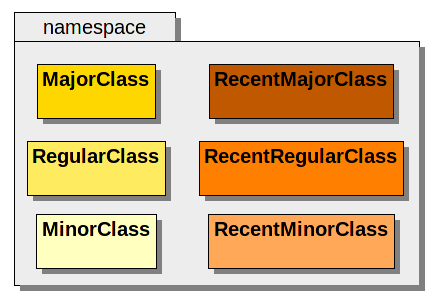
\includegraphics[scale=.33]{../classdiagrams/uml-legend.png}%
\caption{Color conventions in UML diagrams.}%
\label{fig:uml-legend}%
\end{wrapfigure}%

\section{Introduction}

This chapter present the design of \sofa{}, as well as its recent evolutions.
It also includes discussions justifying some of the decision that are behind this design.

The conventions used in UML class diagrams are presented in Fig~\ref{fig:uml-legend}.

\vspace{.8cm}

\section{Core Class Diagrams}

\subsection{Object Model (\textcode{sofa::core::objectmodel})}

\begin{figure}[h]
\centering
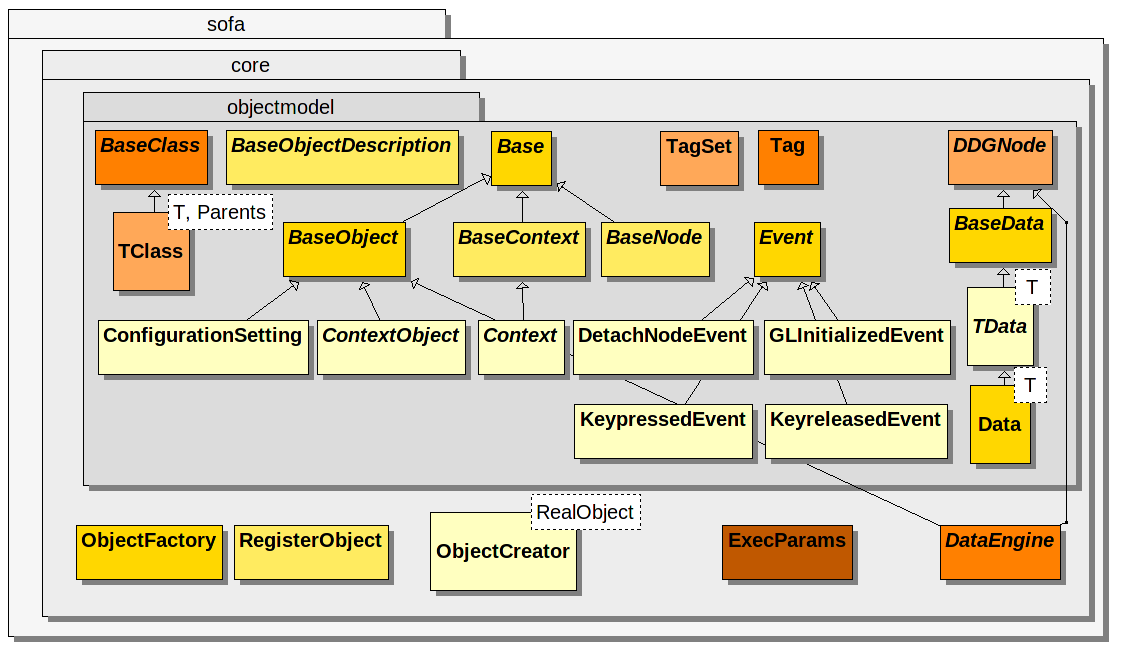
\includegraphics[scale=.33]{../classdiagrams/sofacore-objectmodel.png}
\caption{Classes of the \textcode{sofa::core::objectmodel} namespace.}
\label{fig:uml-sofa-core-objectmodel}
\end{figure}

\subsubsection{Changes compared to the 1.0~beta~4 version}\label{sec:design-core-objectmodel-changes}

\paragraph{New class description system.}
It is based on the \textcode{BaseClass} and \textcode{TClass} classes, and requires to add the \textcode{SOFA\_CLASS} macro in the declaration of all classes deriving from Base.
The benefits are that it is now possible to follow the full hierarchy of classes from the final components, instead of having just a fixed set of categories.
This macro is also necessary in classes with a templated parent class to be able to use methods and member variables defined in \textcode{Base} such as \textcode{initData} or \textcode{sout}. This removed all the previously redundant direct heritage to \textcode{BaseObject} that was previously required.

\paragraph{Objects and node tagging (\textcode{Tag} and \textcode{TagSet}).}
The goal of the introduction of tags is to provide one of the pieces necessary to support non-mechanical states (electrical potentials, constrast agent concentrations) as well as cleaner non-geometrical mechanical states (fluid dynamics, reduced-coordinate articulations).
For example, in a simulation involving blood in deformable vessels, we would use two tags to distinguish the different states : mechanical, fluid.
These tags will be used to easily work with only a subset of the components, so that the mechanical solver works on positions and forcefields but don't interferes with blood flow and pressure, and inversely for the fluid solver\footnote{\url{http://wiki.sofa-framework.org/tdev/wiki/Notes/ProposalGenericStates}}.
We decided on using there tags instead of extending the class hierarchy as was done before with the \textcode{State} and \textcode{MechanicalState} classes.
A hierarchy is fine when we have only one feature that we want to differentiate on (such as base vs mechanical vs electrical), but when we add other criteria (lagrangian geometry vs eulerian vs reduced generalized coordinates, velocity vs vorticity, independent vs mapped DOFs) it is no longer manageable as specialized classes.
A secondary use of these tags is to replace existing subsets mechanisms within CollisionModels (r2441) and Constraints (r3121).
The design is based on the following elements.
Tags are added to BaseObject, as a list of string (internally converted to a list of unique ids for faster processing).
All visitors now filter the objects they process based on their list of tags.
All solvers by default copy their own list of tags to the visitors they execute, so that they only affect the objects with the same tags as they have (TODO: this is currently broken). 

\paragraph{Dependencies between Data (\textcode{DDGNode} and \textcode{DataEngine}).}
The goal is to be able to specify simple links between datas or through computation engines.
To function correctly, the methods \textcode{getValue()} or \textcode{beginEdit()}/\textcode{endEdit()} are required to be called in all codes accessing values contained in Data instances.
To enforce this, the class DataPtr was removed.
Note also that it is very inefficient to call \textcode{getValue()} repetively within computation loops.
Instead, the recommanded method is to use the helper classes \textcode{ReadAccessor} and \textcode{WriteAccessor}
that can hold a reference to a \textcode{Data} value, provides the same API as regular vectors,
and automatically calls \textcode{endEdit()} at the end of the call block in case of \textcode{WriteAccessor}.

\textbf{TODO:} \textit{\textcode{TData<T>} was useful as a common parent for \textcode{Data<T>} and \textcode{DataPtr<T>}, but now that \textcode{DataPtr} no longer exist, it would simplify the hierarchy to merge \textcode{TData<T>} and \textcode{Data<T>}.}

\paragraph{\textit{Copy-on-Write} (CoW) mechanism (\textcode{DataContainer}).}
The goal is to reduce copies of datas when using engines and/or multi-threading.
It is completly transparent to other codes, since everything should now respect the data access API (see above).
There is however one important side-effect that may break some existing code: the pointer to the value of a \textcode{Data} can now change during a call to \textcode{beginEdit()}.
This means that it is now illegal to retrieve the pointer to the value in a \textcode{Data} at init time and then reuse it after edits might have been made.

\paragraph{Support for asynchronous multi-threading (\textcode{ExecParams}).}
This feature is an important goal of the new design, however it is not yet completely functionnal and thus may change shortly.


\subsection{Physical Behavior (\textcode{sofa::core::behavior})}
\begin{figure}[h]
\centering
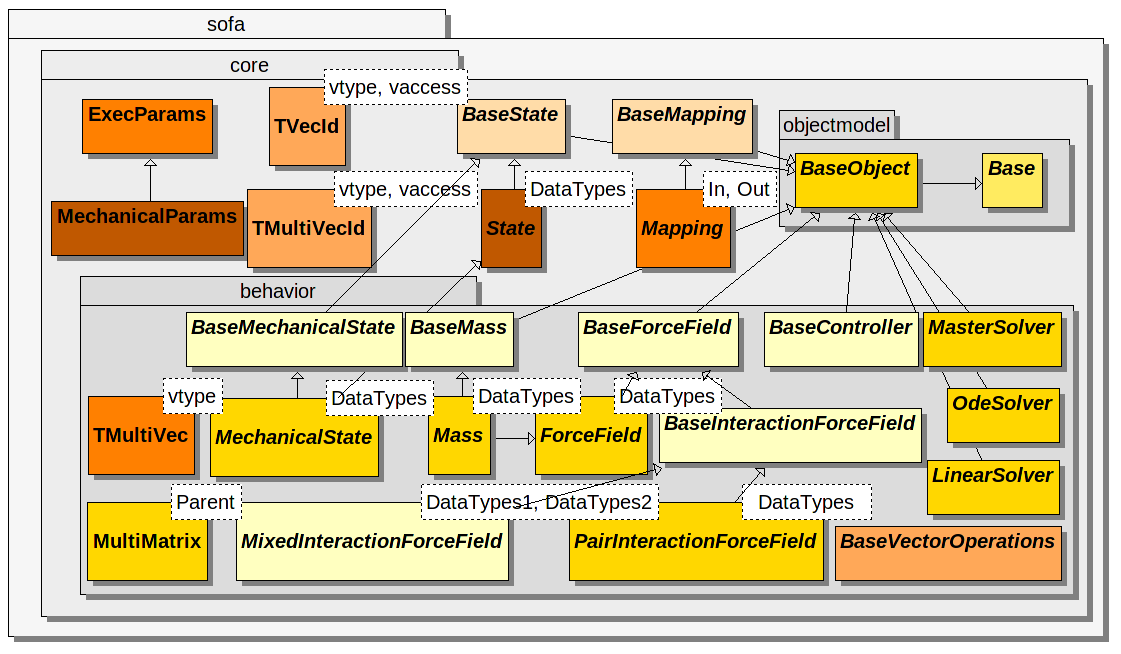
\includegraphics[scale=.33]{../classdiagrams/sofacore-behavior.png}
\caption{Classes of the \textcode{sofa::core::behavior} namespace.}
\label{fig:uml-sofa-core-behavior}
\end{figure}

\subsubsection{Changes compared to the 1.0~beta~4 version}\label{sec:design-core-behavior-changes}

\paragraph{\textcode{VecId} is replaced by templated classes to specify vector types and read/write access.}

Previously, the \textcode{VecId} class was used by solvers and visitors to specify on which state vectors should an operation be applied.
However, this API did not express the requirements for these vectors (which type, i.e. \textcode{Coord}, \textcode{Deriv}, or \textcode{MatDeriv}), nor if they were supposed to be read or written.
Now, methods and visitors can use the following classes instead (all typedefs from a common \textcode{TVecId} templated class), so that developers will now explicitly what to expect:

\begin{code_cpp}
/// Identify one vector stored in State
/// A ConstVecId only provides a read-only access to the underlying vector.
typedef TVecId<V_ALL, V_READ> ConstVecId;

/// Identify one vector stored in State
/// A VecId provides a read-write access to the underlying vector.
typedef TVecId<V_ALL, V_WRITE> VecId;

/// Typedefs for each type of state vectors
typedef TVecId<V_COORD, V_READ> ConstVecCoordId;
typedef TVecId<V_COORD, V_WRITE>     VecCoordId;
typedef TVecId<V_DERIV, V_READ> ConstVecDerivId;
typedef TVecId<V_DERIV, V_WRITE>     VecDerivId;
typedef TVecId<V_MATDERIV, V_READ> ConstMatrixDerivId;
typedef TVecId<V_MATDERIV, V_WRITE>     MatrixDerivId;
\end{code_cpp}

Also, a new class \textcode{TMultiVecId} is introduced to be able to specify different IDs for specific states or groups of states. Similar typedefs are defined as above, replacing \textcode{Vec} with \textcode{MultiVec}.

\paragraph{New State API and class hierarchy.}
The previous State API was based on \textcode{getX()}/\textcode{getV()}/... methods that returned pointers to the vectors last specified (using \textcode{setX()}/\textcode{setV()}/... methods) as the current position, velocity, ...
This is now replaced by \textcode{read(ConstVec\textit{TYPE}Id)} and \textcode{write(Vec\textit{TYPE}Id)} methods, where \textcode{\textit{TYPE}} is either \textcode{Coord}, \textcode{Deriv}, or \textcode{MatDeriv}.
These methods return a pointer to a Data instance containing the vector, instead of the vector itself.
This was necessary to respect the Data access API (see section~\ref{sec:design-core-objectmodel-changes}).
For compatibility with existing codes (especially \textcode{draw()} methods), the read-only \textcode{getX()}/\textcode{getV()}/... methods still exists but they are deprecated (and there are strictly equivalent to calling \textcode{read()} with the default ID for position, velocity, ...).
The non-const versions however are removed, so all codes modifying state vectors will have to use the new Data-based API.
Note that with this change, the state components no longer store the information about which vectors should be considered as the current position, velocity, ...
So another mechanism is required to specify these associations (\textcode{MechanicalParams}, see below).

A new state class hierarchy is also defined,  introducing a new parent class \textcode{BaseState}, common to all states (mechanical, visual, ...).
Methods allowing to read and write vectors given their IDs are specified in \textcode{State<DataTypes>}.
The \textcode{MappedModel} class is removed, non-mechanical state components (such as visual models) now directly derive from \textcode{State<DataTypes>}.


\paragraph{Simplified \textcode{Mapping} class hierarchy.}
Previously, a different base class (\textcode{Mapping< State<TIn>, MappedModel<TOut> >} or \textcode{MechanicalMapping< MechanicalState<TIn>, MechanicalState<TOut> >}) where used for mechanical versus non-mechanical (i.e. visual or one-way) mappings.
This introduced complexities and redundancies in the code of the final components (they where templated by the type of their parent class and compiled twice for each pair of input/output datatypes).
Now, a single base class is used (\textcode{Mapping<TIn,TOut>}, templated only by the input and output datatypes.
Components are also templated by the same types, similarly to other classes such as forcefields.
A new set of flags is used to check if a given mapping is mechanical or not.
Different flags are used to activate the mapping of forces, masses, and constraints separatly (although by default they have the same value).
Components that do not implement applyJT (i.e. visual mappings) can force them to false to indicate they do not support mechanical computations.

\paragraph{New mechanical component API based on \textcode{Data} and \textcode{MechanicalParams}.}
This is the most important change from the previous design.
To provide all the required vector IDs that where previously stored within each \textcode{MechanicalState} by calls to \textcode{setX()}/... methods, we define a \textcode{MechanicalParam} class.
This class is given to all mechanical-related methods, specified by \textcode{OdeSolver}s and transmitted by \textcode{MechanicalVisitor}s.
It hides the \textcode{VecId} system from most component codes, providing the same abstraction of accessing the current position and velocity vectors as was previously handled within \textcode{MechanicalState}. For example, where a component such as a \textcode{ForceField} implementation used :
\begin{code_cpp}
const VecCoord* x = this->mstate->getX();
\end{code_cpp}
It will now use \textcode{MechanicalParams} as follows :
\begin{code_cpp}
helper::ReadAccessor<VecCoord> x = *mparams->readX(this->mstate);
\end{code_cpp}

This API is preferable to directly manipulating \textcode{VecId}s (such as in \textcode{this->mstate->read(mparams->getXId(this->mstate))}) because :
\begin{itemize}
\item The code is very similar to the previous version.
\item If the API of the \textcode{VecId} or \textcode{MechanicalState} class is further changed, the \textcode{MechanicalParam::readX()} method can handle it.
\item Different \textcode{VecId}s for different states can be chosen within \textcode{MechanicalParam} (such as what is currently used for free vs mapped states, and animated vs external obstacle state).
\end{itemize}

However it is still possible to get the ids (using \textcode{mparams->x().getId(mstate)}).

All vector accesses given though \textcode{MechanicalParams} are read-only.
Vectors actually modified by each method are given as separate \textcode{MultiVecId} parameters.
This is useful to make the API clearer (we can see explicitly what each method is supposed to write) and safer (no accidental modifications to X or V within \textcode{addForce()} or \textcode{draw()} for example).
Finally, other interesting pieces of information can be queried though \textcode{MechanicalParams}.
For example, a ForceField can know as soon as the \textcode{addForce()} call if the current solver is implicit or explicit, if the kinematic and potential energy should be computed, ...

\paragraph{New solver hierarchy and vector manipulation API (\textcode{TMultiVec} and \textcode{BaseVectorOperations}).}
Previously, the solver classes had a complex hierarchy, with several parent classes (\textcode{SolverImpl}, \textcode{OdeSolverImpl}, \textcode{MasterSolverImpl}) that where used to launch each type of visitors (mechanics, linear algebra, ...).
In the new design, these classes are replaced by separate helper classes (\textcode{VectorOperations}, \textcode{MechanicalOperations}) that are instanciated at runtime and allow to launch each type of visitors while holding and updating the persistant parameters (in the form of a \textcode{MechanicalParams} for mechanical visitors for example, or \textcode{ExecParams} for simple vector operations).


\subsection{Topology (\textcode{sofa::core::topology})}

\textit{The design of this namespace is still a work in progress, so major changes should still be expected...}

\subsubsection{Changes compared to the 1.0~beta~4 version}

\textit{To be documented...}

\subsection{Collision (\textcode{sofa::core::collision})}

\begin{figure}[h]
\centering
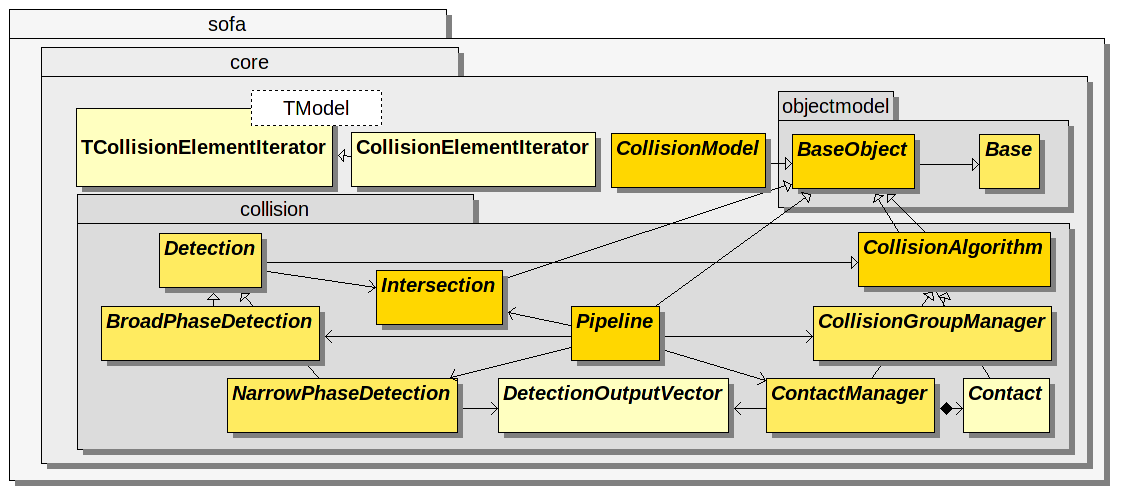
\includegraphics[scale=.33]{../classdiagrams/sofacore-collision.png}
\caption{Classes of the \textcode{sofa::core::collision} namespace.}
\label{fig:uml-sofa-core-collision}
\end{figure}

\subsubsection{Changes compared to the 1.0~beta~4 version}

\textit{No major changes.}

\subsection{Mesh and Image Loaders (\textcode{sofa::core::loader})}

\begin{figure}[h]
\centering
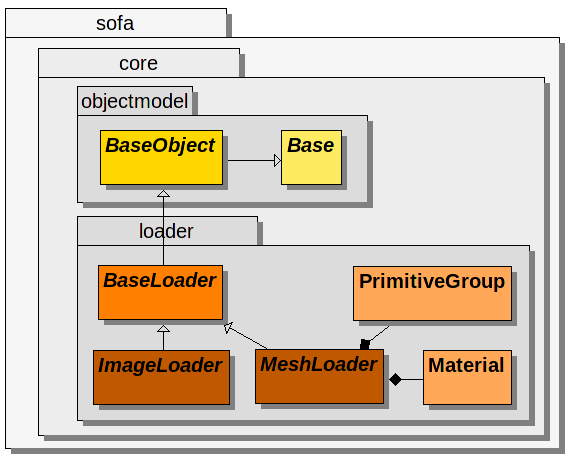
\includegraphics[scale=.33]{../classdiagrams/sofacore-loader.png}
\caption{Classes of the \textcode{sofa::core::loader} namespace.}
\label{fig:uml-sofa-core-loader}
\end{figure}

\subsubsection{Changes compared to the 1.0~beta~4 version}

This namespace is completely new.

\textit{To be documented...}

\pagebreak

\section{Main classes}

\subsection{\textcode{sofa::core::objectmodel}}

\subsubsection{\textcode{Base}}

\lstinputlisting[style=C++,linerange=51-181]{../../framework/sofa/core/objectmodel/Base.h}

\subsubsection{\textcode{BaseObject}}

\lstinputlisting[style=C++,linerange=61-160]{../../framework/sofa/core/objectmodel/BaseObject.h}

\subsection{\textcode{sofa::core}}

\subsubsection{\textcode{BaseState}}

\lstinputlisting[style=C++,linerange=39-58]{../../framework/sofa/core/BaseState.h}

\subsubsection{\textcode{State}}

\lstinputlisting[style=C++,linerange=38-103]{../../framework/sofa/core/State.h}

\subsubsection{\textcode{BaseMapping}}

\lstinputlisting[style=C++,linerange=48-116]{../../framework/sofa/core/BaseMapping.h}

\subsubsection{\textcode{Mapping}}

\lstinputlisting[style=C++,linerange=43-115]{../../framework/sofa/core/Mapping.h}


%% \section{Framework}

%% \subsection{UML Diagrams}

%% \begin{figure}[h]
%% \centering
%% 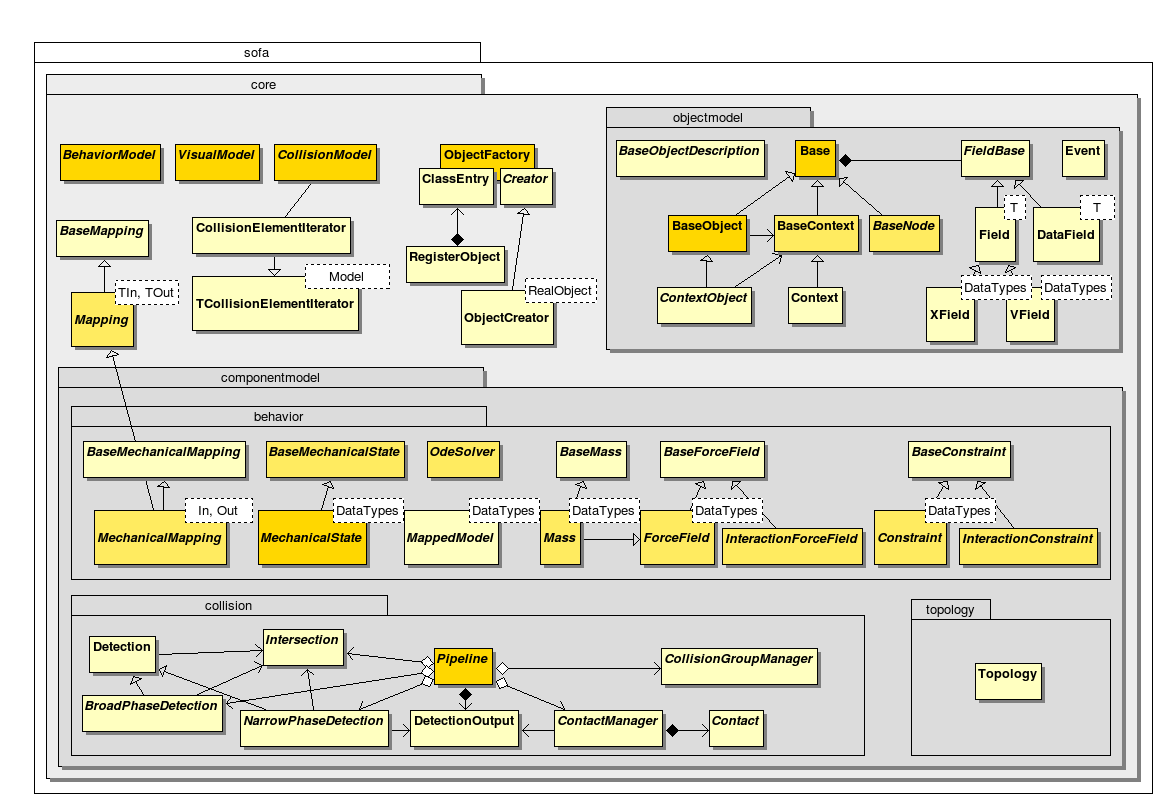
\includegraphics[width=\linewidth]{uml-sofa-core.png}
%% \caption{Classes of the sofa::core namespace.}
%% \label{fig:uml-sofa-core}
%% \end{figure}

\chapter{Modules}
\graphicspath{{modules/}}  % to include images
In this document we explain the usage and the fucntionalities of the modules developped using the Core Sofa Framework.
\section{Collision Models}
\subsection{Ray Traced Collision Detection}
This module implements the algorithm described in the paper entitled "Ray-traced collision detection for deformable bodies" by E.Hermann F.Faure and B.Raffin. When two objects are in collision, a ray is shot from each surface vertex in the direction of the inward normal. A collision is detected when the first intersection belongs to an inward surface triangle of another body.  A contact force between the vertex and the matching point is then created. Experiments  show that this approach is fast and more robust than traditional proximity-based collisions.

 To speedup the  searching of elements that cross the ray,   we  stored all the triangles of each colliding objects in an  octree. Therefore we can easily navigate inside this octree and efficiently find the points crossing the ray. The octree structure allow us to have a satisfying performance independently from the size of the triangles used, which is not the case for  a regular grid.


\subsubsection{Using this module}
An example showing the usage of the Ray Traced collision detection can be found in the  RayTraceCollision.scn file in the \textit{scene} directory. The collision detection mechanism must be set as \textbf{RayTraceDetection}, and instead of using a TriangleModel one must use a \textbf{TriangleOctreeModel}. The TriangleOctreeModel will create an Octree that contains all the Triangles from the collision model. 
	


\newpage
\section{Soft Articulations}


\subsection{Concepts}

The objective of this method is to use stiff forces to simulate joint articulations, instead of classical constraints.
\paragraph{}
To do this, a joint is modeled by a 6 degrees of freedom spring. By the way, the user specify a stiffness on each translation and rotation.
\begin{itemize}
	\item A null stiffness defines a free movement.
	\item A huge stiffness defines a forbidden movement.
	\item All nuances are possible to define semi constrained movements.
\end{itemize}

\paragraph{}
2 main advantages can be extracted from this method :
\begin{itemize}
	\item A better stability. As we don't try to statisfy constraints but only apply forces, there is always a solution to resolve the system.
	\item more possibilities to model articulations are allowed. As the stiffnesses define the degrees of freedom of the articulations, a better accuracy is posssible to simulate free movements as forbidden movements, i.e. an articulation axis is not inevitably totally free or totally fixed.
\end{itemize}



\subsection{Realization}

To define physically an articulated body, we first have a set of rigids (the bones). \textsl{cf fig. 1}
\begin{figure}[hp]
	\centering
		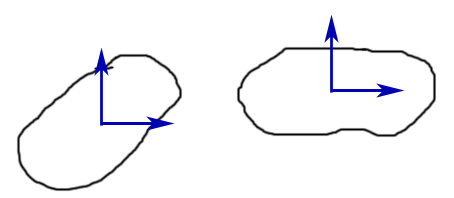
\includegraphics[width=0.30\textwidth]{softArt_G1.png}
	\caption{two bones}
	\label{2 Bones}
\end{figure}


Each of these bones contains several articulations points, also defined by rigids to have orientation information. \textsl{cf fig. 2}
\begin{figure}[htpb]
	\centering
		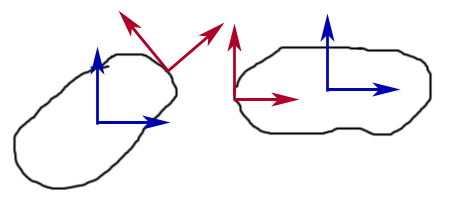
\includegraphics[width=0.30\textwidth]{softArt_G2.png}
	\caption{two bones (blue) with their articulation frames (red)}
\end{figure}

As seen previously, a joint between 2 bones is modeled by a 6-DOF spring. These springs are attached on the articulations points.    \textsl{cf fig. 3}
\begin{figure}[htpb]
	\centering
		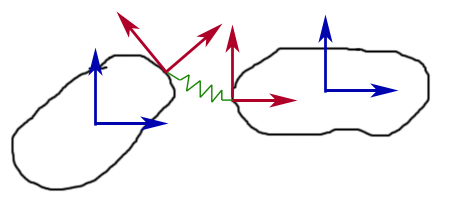
\includegraphics[width=0.30\textwidth]{softArt_G3.png}
	\caption{two bones linked by a joint-spring}
\end{figure}



\subsection{Sofa implementation}

To simulate these components in Sofa, we first need 2 mechanical objects : one for the bones (independent DOFs), and an other for the articulation points (mapped DOFs).
Each of them contains a list of rigid DOFs (respectively all the bones and all the articulations of the articulated body).
A mapping performs the link between the two lists, to know which articulations belong to which bones.


\subsubsection{Corresponding scene graph}
\begin{figure}[htpb]
	\centering
		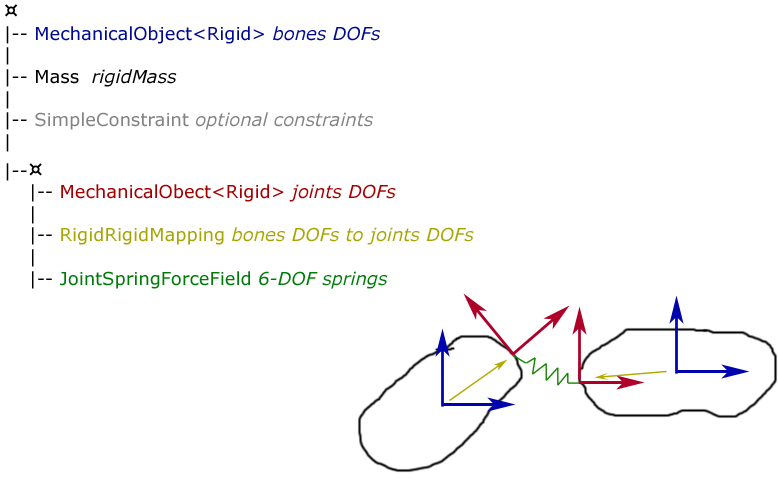
\includegraphics[width=0.90\textwidth]{scene_graph.png}
	\caption{a simple articulated body scene}
\end{figure}

\subsubsection {Example}

The example softArticulations.scn shows a basic pendulum :

\begin{verbatim}
<Node>
  <Object type="BruteForceDetection"/>
  <Object type="DefaultContactManager"/>
  <Object type="DefaultPipeline"/>
  <Object type="ProximityIntersection"/>

  <Node>
    <Object type="CGImplicitSolver"	/>
    <Object type="MechanicalObject" template="Rigid" name="bones DOFs"
            position="0 0 0  0 0 0 1 
                      1 0 0  0 0 0 1 
                      3 0 0  0 0 0 1 
                      5 0 0  0 0 0 1 
                      7 0 0  0 0 0 1" />
    <Object type="UniformMass" template="Rigid" name="bones mass"
            mass="1 1 [1 0 0,0 1 0,0 0 1]" />
    <Object type="FixedConstraint" template="Rigid" name="fixOrigin"
            indices="0" />
		
    <Node>
      <Object type="MechanicalObject" template="Rigid" name="articulation points"
              position="0 0 0  0.707914 0 0 0.707914 
                       -1 0 0  0.707914 0 0 0.707914 
                        1 0 0  0.707914 0 0 0.707914 
                       -1 0 0  0.707914 0 0 0.707914 
                        1 0 0  0.707914 0 0 0.707914 
                       -1 0 0  0.707914 0 0 0.707914 
                        1 0 0  0.707914 0 0 0.707914 
                       -1 0 0  0.707914 0 0 0.707914 
                        1 0 0  0.707914 0 0 0.707914" />
      <Object type="RigidRigidMapping"
              repartition="1 2 2 2 2" />
      <Object type="JointSpringForceField" template="Rigid" name="joint springs"
              spring="0 1   0 0 0 0 1 0   0 30000  0 200000   0  0 0 0  0 0 0 1 
                      2 3   0 0 0 0 1 0   0 30000  0 200000   0  0 0 0  0 0 0 1
                      4 5   0 0 0 0 1 0   0 30000  0 200000   0  0 0 0  0 0 0 1
                      6 7   0 0 0 0 1 0   0 30000  0 200000   0  0 0 0  0 0 0 1" />
    </Node>
    <Node>
      <Object type="MechanicalObject" template="Vec3d"
              position="-1 -0.5 -0.5  -1 0.5 -0.5 ..." />
      <Object type="MeshTopology"
              lines="0 1  1 2  ..."
              triangles="3 1 0  3 2 1  ..." />
      <Object type="TriangleModel"/>
      <Object type="LineModel"/>
      <Object type="RigidMapping"
              repartition="0 8 8 8 8" />
    </Node>
  </Node>
</Node>

\end{verbatim}

\begin{figure}[htpb]
	\centering
		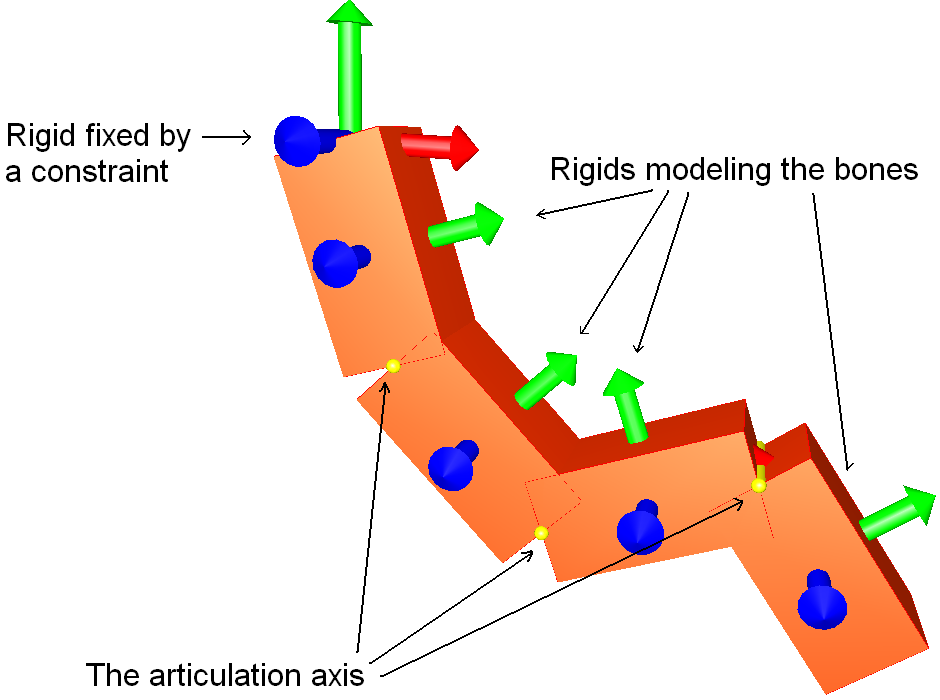
\includegraphics[width=0.70\textwidth]{softArt_snapshot.png}
	\caption{The pendulum is composed by 4 rigids linked one by one by articulations}
\end{figure}

In this example, we have under the first node the components to manage collisions, as usual.
Under the second node, we have :
\begin{itemize}
	\item the solver,
	\item the mechanical object modeling the independent rigid DOFs (5 rigids here),
	\item the rigid mass,
	\item a constraint, to fix the first rigid.
\end{itemize}

The third node (a child of the previous one) contains the components relative to the articulations :
\begin{itemize}
	\item the mechanical object modeling articulation points. Positions and orientations are relative to their parents.
	\item the mapping to link the two mechanical objects, as explained before. To know which articulations belong to which bones, a repartition vector is used. Several cases for this vector are possible :
		\begin{itemize}
			\item no value specified : every articulations belong to the first bone (classic rigid mapping).
			\item one value specified (ex: repartition="2") : each bone has the same number of articulations.
			\item number of bones values (like here, repartition="1 2 2 2 2") : the number of articulations is specified for each bone. For instance, here the first bone has 1 articulation, the next has 2 articulations, the next 2, Etc.
		\end{itemize}
	\item the JointSpringForceField containing the springs (4 springs here). Each spring is defined by a list of parameters. For instance for the first spring we have "0 1   0 0 0 0 1 0   0 30000  0 200000   0  0 0 0  0 0 0 1".
		\begin{itemize}
			\item "0 1" are the indices of the two articulations the spring is attached to
			\item "0 0 0 0 1 0" design the free axis for the movements. "0 0 0" mean that the 3 translation axis are constrained, and "0 1 0" mean that only the Y rotation axis is free.
			\item "0 30000 0 2000000" are the stiffnesses for each kind of movement: "0 30000" are respectively for free translation and for constrained translation", and "0 2000000" are respectively for free rotation and for constrained rotation.
			\item "0" is the damping factor
			\item "0 0 0" is to specify the initial translation
			\item "0 0 0 1" is to specify the initial rotation (quaternion)
		\end{itemize}
\end{itemize}

The last node contains the collision model. Nothing special here.


\subsection{Skinning}

The articulated body described previously models the skeleton of an object.
To have the external model (for the visual model or the collision model), which follows correctly the skeleton movements, it has to be mapped with the skeleton. 
\ 
A skinning mapping allows us to do this link. The external model is from this moment to deform itself smoothly, i.e. without breaking points around the articulations.

The influence of the bones on each point of the external model is given by skinning weights.
2 ways are possible to set the skinning weights to the mapping :
\begin{itemize}
	\item Either the user gives directly the weights list to the mapping. It is useful if good weights have been pre computed previsouly, like in Maya for instance.
	\item Else, the user defines a number of references \textsl{n} that will be used for mapped points. Then, each external model point will search its \textsl{n} nearest bones (mechanical DOFs), and then compute the skinning weights from the relation :
\[ W = \frac{1}{d^{2}}  \]
\small{ with \textsl{d} : the distance between the external point and the rigid DOF.}
\end{itemize}

\begin{figure*}[htpb]
		\centering
		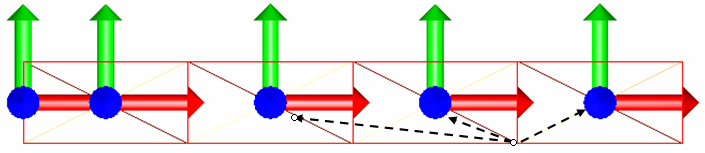
\includegraphics[width=0.50\textwidth]{skinning}
		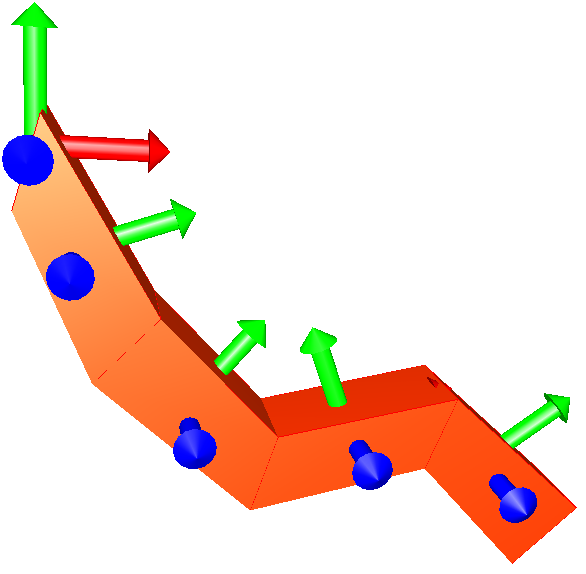
\includegraphics[width=0.30\textwidth]{skinnedPendulum}	
	\caption{In the example "softArticulationsSkinned.scn" the external points compute their skinning weights from the 3 nearest DOFs}
\end{figure*}

\newpage
\section{How to use mesh topologies in SOFA}

H. Delingette, B. Andr�

\subsection{Introduction}

\subsubsection{BTW, What is a mesh topology ?}

A mesh is usually described as a set of points that are connected by
edges, triangles or any other type of mesh element. Thus it is
useful to make a clear a distinction between two different aspects
of a mesh :

\begin{itemize}

 \item \textbf{Mesh Geometry} : the mesh geometry consists in the position of the mesh vertices.
This information depends on the space where the mesh in embedded.
For instance in a 2D triangulation, each vertex position is a 2D
vector while in a 3D triangulation, each vertex position is a 3D
vector. Therefore the mesh geometry can be described as an array of
vector whose size is the number of mesh vertices. In SOFA, we use
the word Degree Of Freedom (DOF) to describe such an array because
it can be used to store other geometric information (rigid
transformation, first or second derivatives, etc.).

 \item \textbf{Mesh Topology} : the mesh topology describes how the vertices are
connected with each other. For instance, it describes the set of
triangles by specifying the 3 vertex indices that make each
triangle. A mesh topology manipulates vertex indices (as unsigned
int) and therefore is independent of the embedding space. For
instance, a 2D and a 3D triangulation may have the same mesh
topology but with different mesh geometry.

\end{itemize}


\subsubsection{Why do I need to bother with mesh topologies ?}

As discuss above, mesh topology is an essential part of a mesh and
therefore any computation task that requires a mesh needs to know
how to use a mesh topology.\\ This includes:

\begin{itemize}

 \item \textbf{Mesh Visualization},

 \item \textbf{Collision detection} : some collision detection are mesh based (e.g.
triangles or edges),

 \item \textbf{Mechanical Modeling} : deforming a mesh also requires to the
knowledge of a mesh topology. For instance a spring mass model
requires knowing about the edges that connects pair of vertices,

 \item \textbf{Haptic rendering},

 \item \textbf{Description of scalar} (temperature, electric potential, etc.) or
vectorial fields (speed, fiber orientation, etc.)

\end{itemize}

Using a mesh topology is relatively simple since it consists in
having access to arrays of indices corresponding to vertex indices
or edge indices or other topological items.
\\

A more tricky part consists a) in changing locally or globally this
topology (adding a triangle, removing an edge) and b) in propagating
those changes to all objects using the mesh topology to perform a
task (visualization, deformation, etc.)

\subsubsection{How are Mesh Topologies designed in SOFA ?}

The mesh geometry in SOFA is stored in a MechanicalObject which is a
template class because it depends on the embedding space (2D or 3D
Euclidian space), the vector class and the required floating point
accuracy (float vs double).
\\

A mesh topology is stored in a different object than the mesh
geometry.
\\

One important aspect of the design of mesh topologies in SOFA is the
fact that they are organized in a class hierarchy. For instance, a
triangulation object derives from an edge set object since a
triangulation can be also viewed as a set of edges, each triangle
having 3 edges. This is very important to design generic software
components. Indeed, following the same example, with this design, a
spring mass mechanical model that only requires the knowledge of
edges (pairs of vertices) can also be used on a triangulation or any
other mesh (quad, hexahedral, tetrahedral mesh)  that derives from
an edge set object.
\\

Another interesting feature in SOFA is the ability to provide
multiple topology descriptions for the same mesh. For instance a
quad element (see figure below) has four DOFs which can be connected
with 2 triangles or 6 edges. Thus, the same mesh geometry can be
described by 3 different mesh topologies. SOFA uses the mechanism of
topological mapping to provide multiple topologies associated with
the same mesh geometry. Those mappings also apply to map a subset of
the mesh topology into a new mesh topology.  For instance the border
of a tetrahedral mesh can be mapped into triangulation mesh or edges
of a triangulated mesh can be mapped into a polygonal mesh.\\


\begin{figure*}
 \centering
 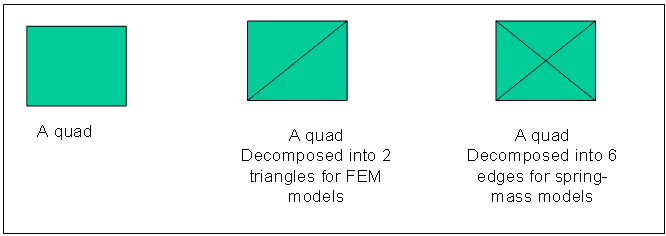
\includegraphics[width=0.95\linewidth]{Quad_Multiple_Topologies}
  \caption{Multiple topology descriptions of the Quad.}
 \label{fig:Quad_Multiple_Topologies}
\end{figure*}

Another important aspect of the design is the fact that topological
changes (mesh cutting or refinement) are handled in SOFA.  For the
programmer, it implies that specific containers must be used to
store data for each software component. For instance, a spring mass
model must store the spring stiffness of each edge. Therefore the
container of spring stiffness must have the same size than the
number of edges in the mesh. In SOFA, to cope with topological
changes that can add or remove the number of edges, it is mandatory
to use a specific container (in such case EdgeData container) that
will automatically resize itself when topological changes occur.

\subsubsection{What are the different mesh topologies supported in SOFA ?}


\subsection{Using Mesh Topologies}

\subsubsection{What is a mesh topology object ?}
\subsubsection{What is the difference with the old MeshTopology object ?}
\subsubsection{What are the different mesh topology objects in SOFA ?}


\begin{figure*}
 \centering
 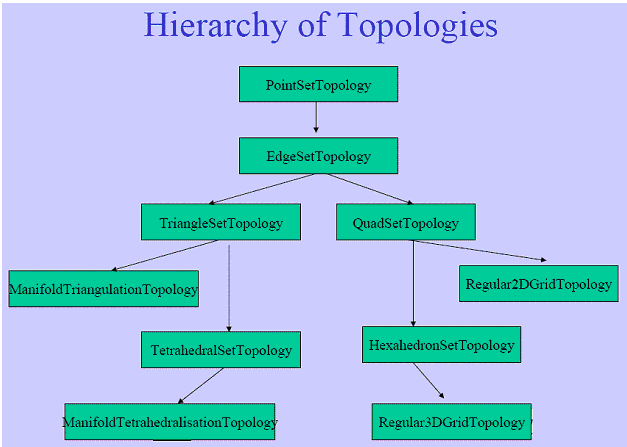
\includegraphics[width=0.95\linewidth]{Hierarchy_Topologies}
  \caption{A generic and hierarchical topology is described from a class called BaseTopology.}
 \label{fig:Hierarchy_Topologies}
\end{figure*}

BaseTopology class provides an implementation which handles
topological changes, full topological relationships and geometric
computation.

\subsubsection{How do I have access to the adjacency information between items ?}
\subsubsection{What to do if I need to know only basic topology information ?}
\subsubsection{What are the geometry algorithms stored in each topology classes ?}

\subsection{Handling Topological Changes}

\subsubsection{How does it work ?}
\subsubsection{What container should I use to handle the topology changes ?}
\subsubsection{How to write the different callback functions associated with the containers ?}

Topological changes are handled in a way which is as much
transparent for the user as possible.


\subsubsection{The 4 components of a BaseTopology object}

\begin{verbatim}

Class BaseTopology<DataTypes> {

// A container for info to be stored and methods to access adjacency :
//   - Adjacency Information is only computed when needed
//   - Non template class
//   - Store TopologicalChange list

TopologyContainer *container ;

// A modifier for low-level methods to change topology :
//   - Cannot be accessed from user
//   - Modifier also changes the DOFs in the Mechanical Object
//   - Low level methods to add or to remove an item
TopologyModifiers<DataTypes> *modifier ;

// TopologyAlgorithms for high-level methods to change topology (user access) :
//   - Accessed from the user
//   - High level algorithms to refine, cut mesh
TopologyAlgorithms<DataTypes> *topologyAlgorithms ;

// Geometry Algorithms methods to get geometry information :
//   - Compute geometric information (normal, curvature, area, length)
GeometryAlgorithms<DataTypes> *geometryAlgorithms ;

};

\end{verbatim}


\subsubsection{Implementation for objects inherited from each other (Point,
Edge, Triangle, Tetrahedron}


\begin{itemize}

 \item PointSetTopology (inherited from BaseTopology) :

    \begin{itemize}

    \item Container : For each point gives its global index. This is useful for subset topologies (subset triangulation, ...) where the number of vertices involved in the topology may not be the same as the total number of vertices.

    \item Modifier : addPointsProcess, removePointsProcess, renumberPointsProcess, addPointsWarning, removePointsWarning, propagateTopologicalChanges

    \item Geometry : computeCenter, computeRadius,
    getAABB()

    \end{itemize}


\item EdgeSetTopology (inherited from PointSetTopology)

    \begin{itemize}

    \item Container : array of edges, array of vertex-edge shell

    \item Modifier : addEdgesProcess, removeEdgesProcess, fuseEdgesProcess, splitEdgesProcess,
   addEdgesWarning, removeEdgesWarning

    \item Geometry : getEdgeLength, getRestEdgeLength

    \end{itemize}


\item TriangleSetTopology (inherited from EdgeSetTopology)

    \begin{itemize}

    \item Container : array of triangles, of vertex- and edge-triangle shell

    \item Modifier : addTrianglesProcess, removeTrianglesProcess, addTrianglesWarning, removeTrianglesWarning

    \item Topology Algorithms : InciseAlongPointsList, RemoveAlongTrianglesList

    \item Geometry : computeTriangleNormal

    \end{itemize}


\item TetrahedronSetTopology (inherited from TriangleSetTopology)

    \begin{itemize}

    \item Container : array of tetrahedra, array of vertex-, edge-, triangle-tetrahedra shell

    \item Modifier : addTetrahedraProcess, removeTetrahedraProcess, addTetrahedraWarning, removeTetrahedraWarning

    \item Geometry : computeTetrahedronVolume

    \end{itemize}

\end{itemize}

\begin{figure*}
 \centering
 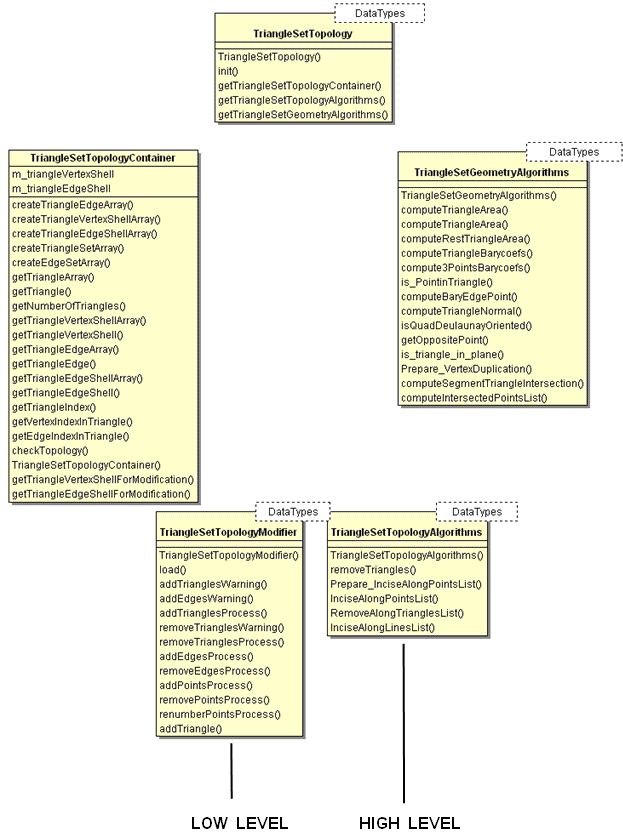
\includegraphics[width=0.95\linewidth]{UML_TriangleSetTopology}
  \caption{UML diagram describing the 4 components of TriangleSetTopology class.}
 \label{fig:UML_TriangleSetTopology}
\end{figure*}

\newpage

\begin{figure*}
 \centering
 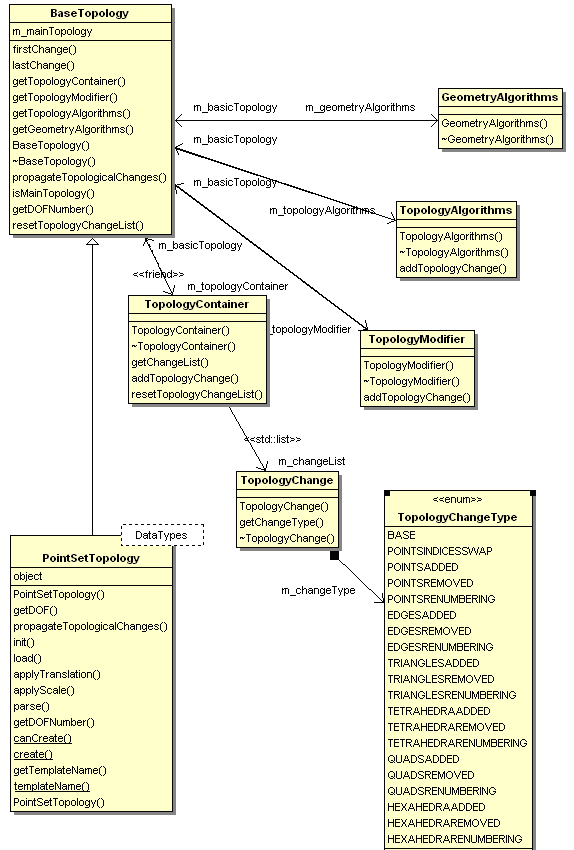
\includegraphics[width=0.95\linewidth]{UML_BaseTopology}
  \caption{UML diagram showing the use of a TopologyChanges List from BaseTopology class.}
 \label{fig:UML_BaseTopology}
\end{figure*}

\newpage

\subsubsection{Definition of data structures to be "aware" of topological
changes}

Force Fields, Constraints, Mapping and other modules may require to
store information for each topological item (point, edge, triangle,
etc.).
\\

Two container data structures are defined to handle topological
changes by matching the types of TopologyChanges :

\begin{itemize}

    \item PointData$<$MyType$>$, EdgeData$<$MyType$>$ are arrays (same as std::vector) of item of type MyType

    \item PointSubset, EdgeSubset are arrays of points or edges

\end{itemize}

Used-defined functions are called when an item is created or
destroyed.
\\

In higher level classes (for example
TriangularQuadraticSpringForceField, DiagonalMass or FixedConstraint
classes), the user only provides callback functions to handle :

\begin{itemize}

    \item the creation of a topological item
    \item the destruction of a topological item

\end{itemize}

\begin{figure*}
 \centering
 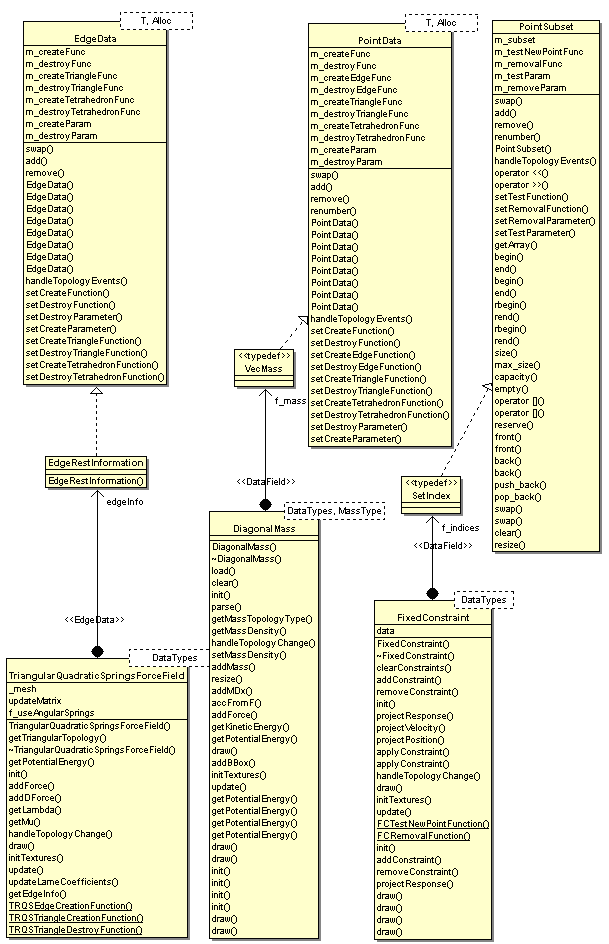
\includegraphics[width=0.95\linewidth, height=0.95\textheight]{UML_Topological_Changes}
  \caption{These UML diagrams show the use of EdgeData, PointData and
PointSubset to handle topological changes implying modifications
respectively in ForceField, Mass and Constraint modules.}
 \label{fig:UML_Topological_Changes}
\end{figure*}

\newpage

\begin{figure*}
 \centering
 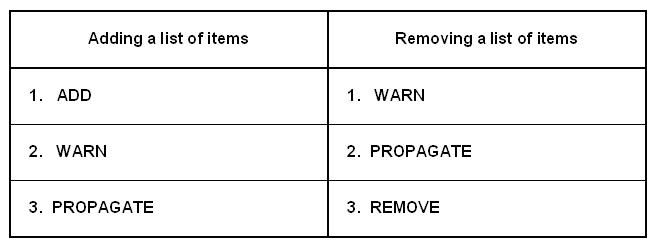
\includegraphics[width=0.95\linewidth]{Order_Notifications}
  \caption{Order to respect when adding or removing an item (see the
explanations in the following example).}
 \label{fig:Order_Notifications}
\end{figure*}

\begin{itemize}

    \item "WARN" means : add the current topological change (add or delete a list of items) in the list of TopologyChanges

    \item "PROPAGATE" means :  traverse the simulation tree with a TopologyChangeVistor to send
    the current topological change event to all force fields, constraints,
    mappings, etc.

\end{itemize}

\subsubsection{Example : What happens when I split an Edge ?}

\begin{figure*}
 \centering
 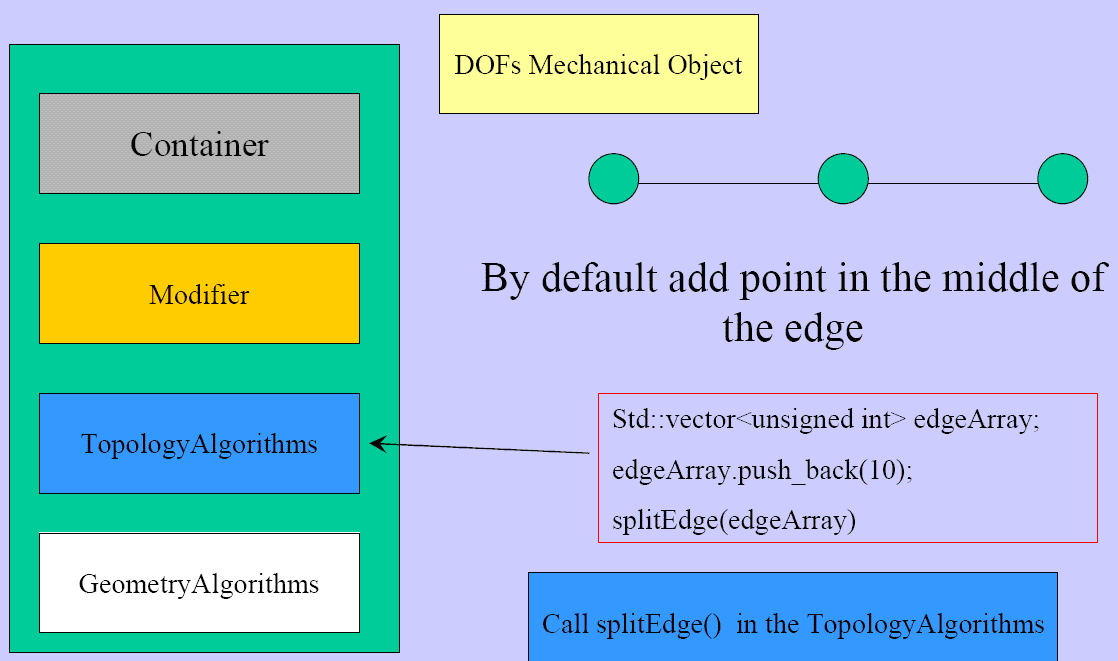
\includegraphics[width=0.95\linewidth]{Topology_Example_1}
 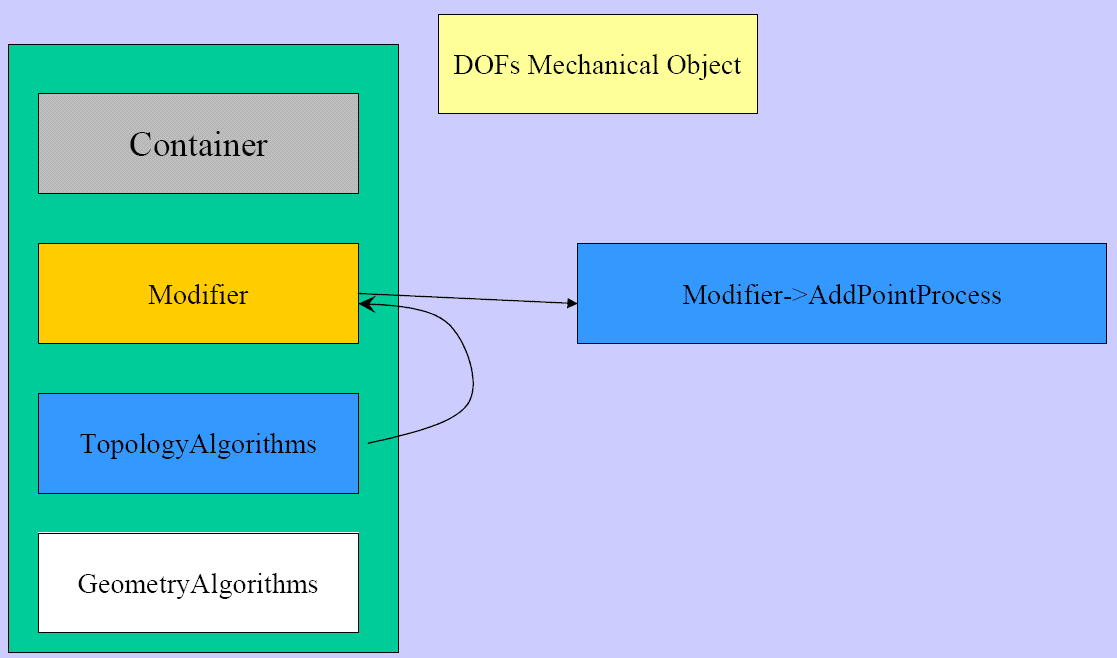
\includegraphics[width=0.95\linewidth]{Topology_Example_2}
  \caption{What happens when I split an Edge ? - Step 1. 2.}
 \label{fig:Topology_Example_12}
\end{figure*}

\newpage

\begin{figure*}
 \centering
 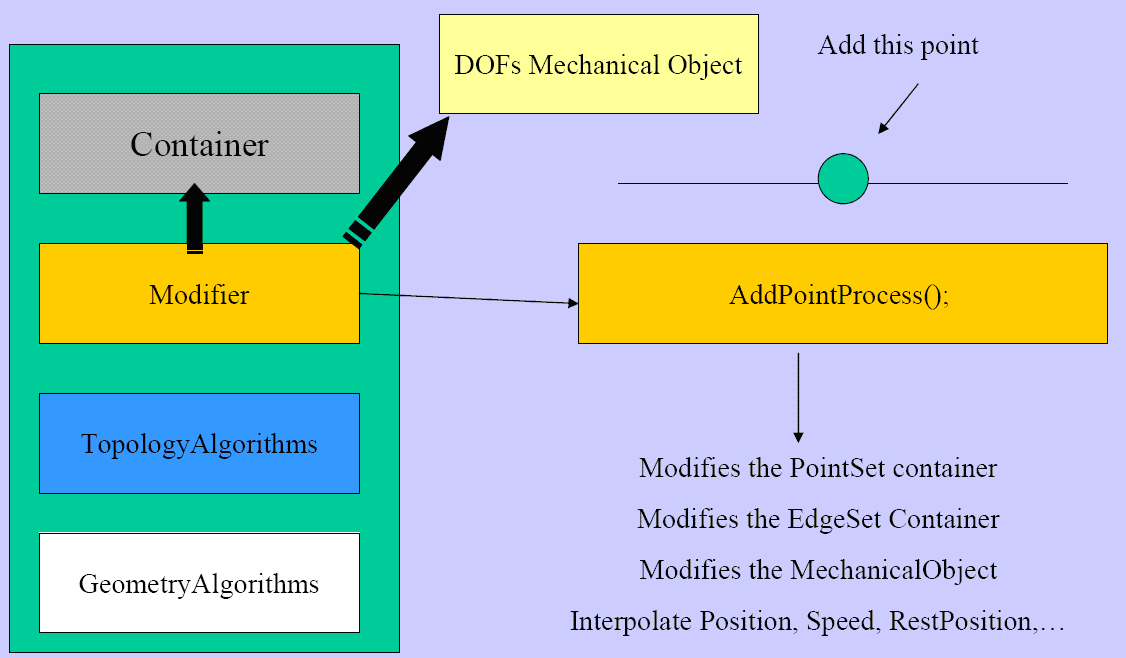
\includegraphics[width=0.95\linewidth]{Topology_Example_3}
 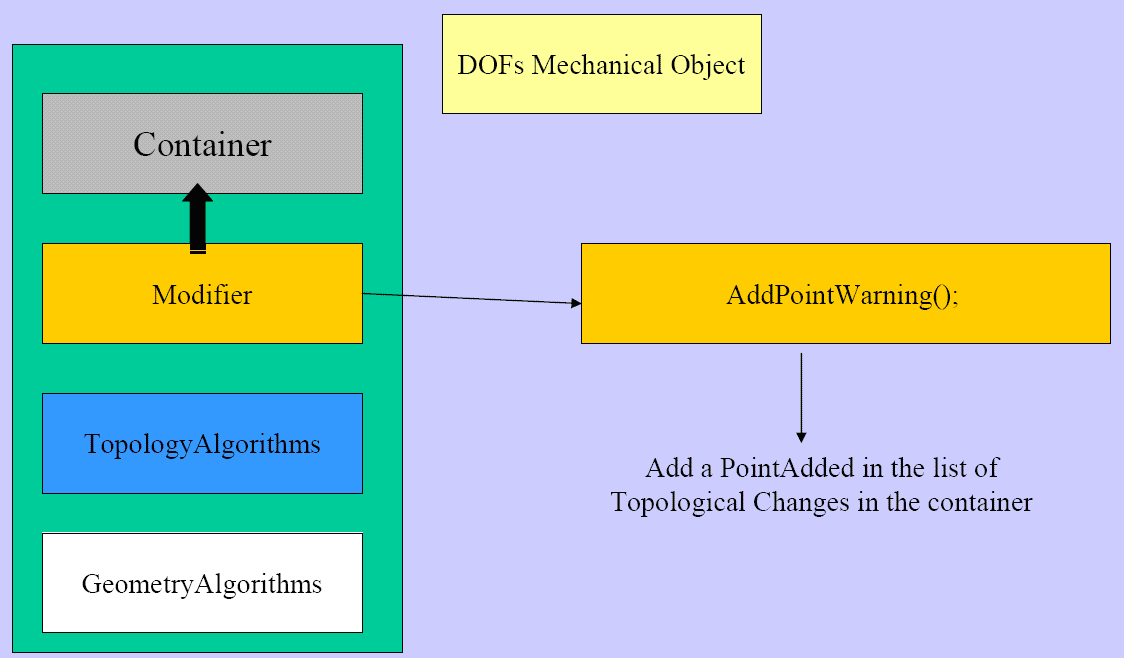
\includegraphics[width=0.95\linewidth]{Topology_Example_4}
  \caption{What happens when I split an Edge ? - Step 3. 4.}
 \label{fig:Topology_Example_34}
\end{figure*}

\newpage

\begin{figure*}
 \centering
 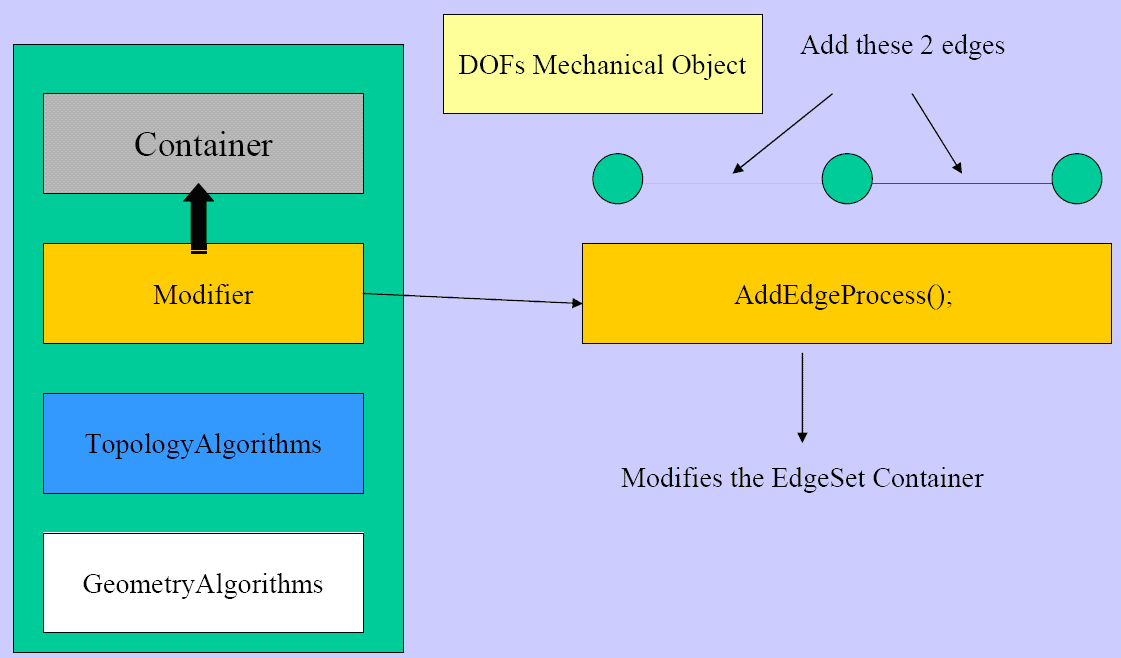
\includegraphics[width=0.95\linewidth]{Topology_Example_5}
 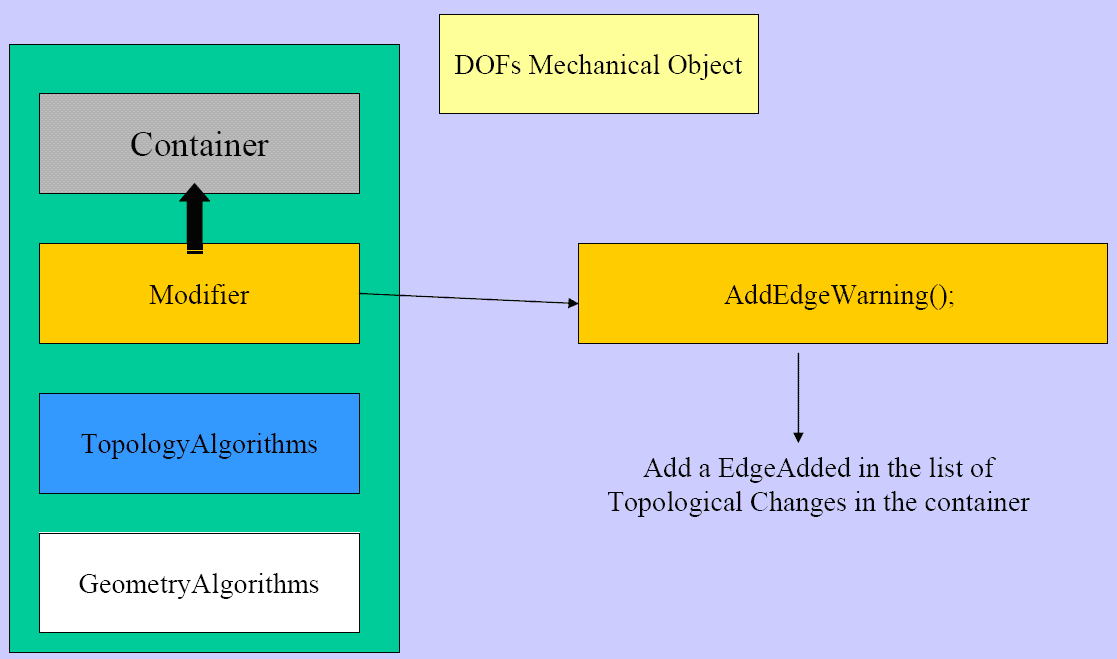
\includegraphics[width=0.95\linewidth]{Topology_Example_6}
  \caption{What happens when I split an Edge ? - Step 5. 6.}
 \label{fig:Topology_Example_56}
\end{figure*}

\newpage

\begin{figure*}
 \centering
 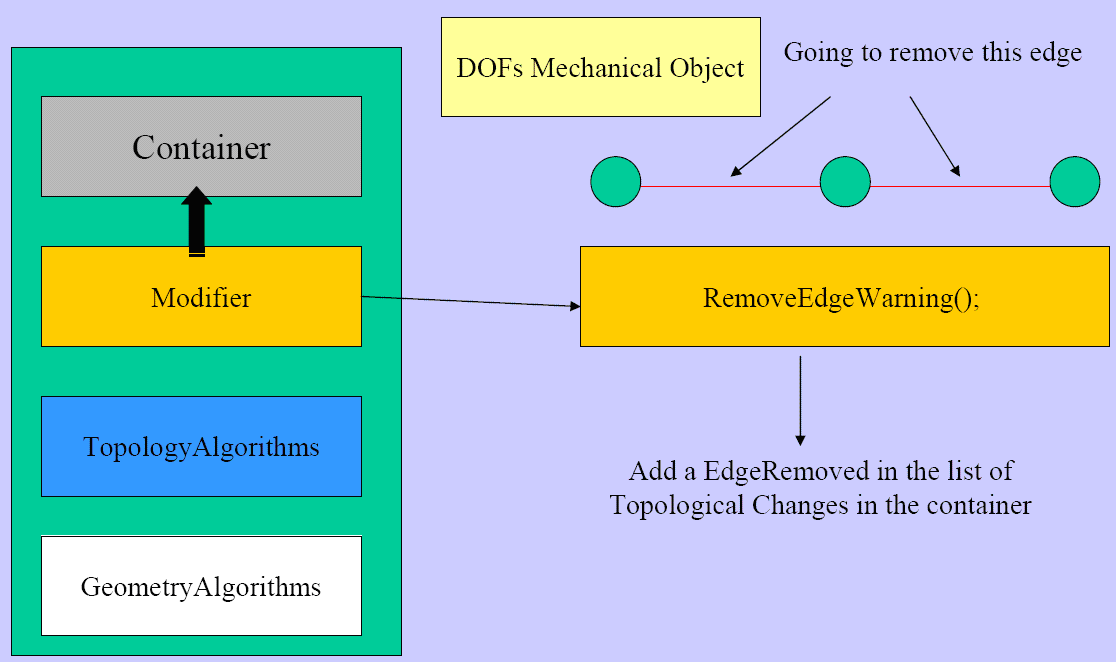
\includegraphics[width=0.95\linewidth]{Topology_Example_7}
 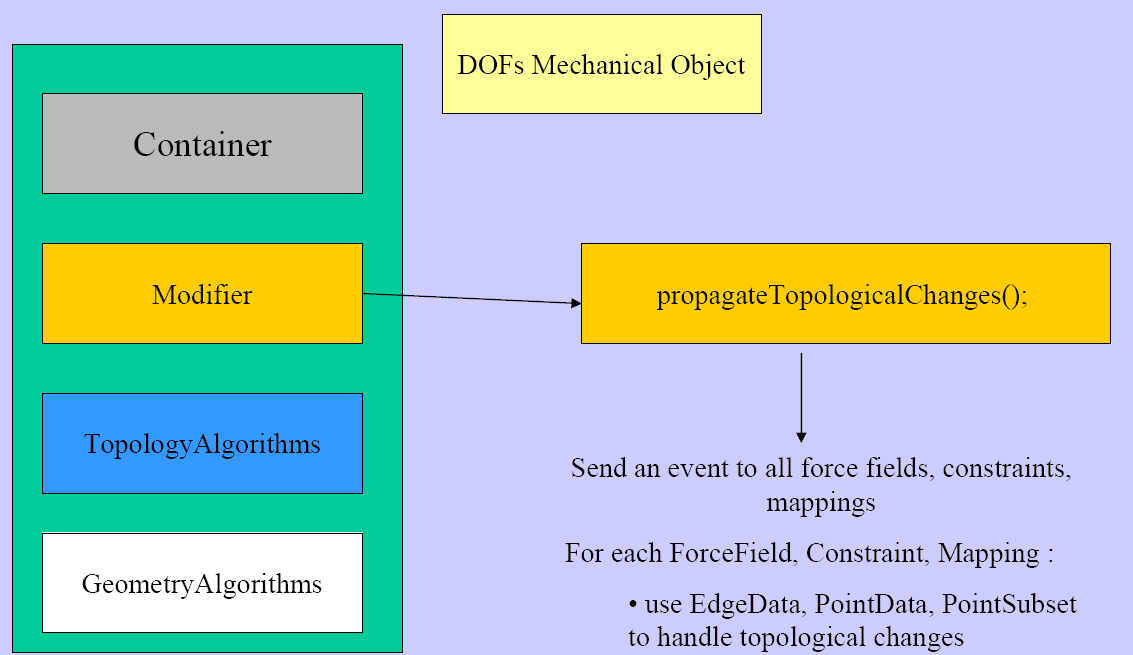
\includegraphics[width=0.95\linewidth]{Topology_Example_8}
  \caption{What happens when I split an Edge ? - Step 7. 8.}
 \label{fig:Topology_Example_78}
\end{figure*}

\newpage

\begin{figure*}
 \centering
 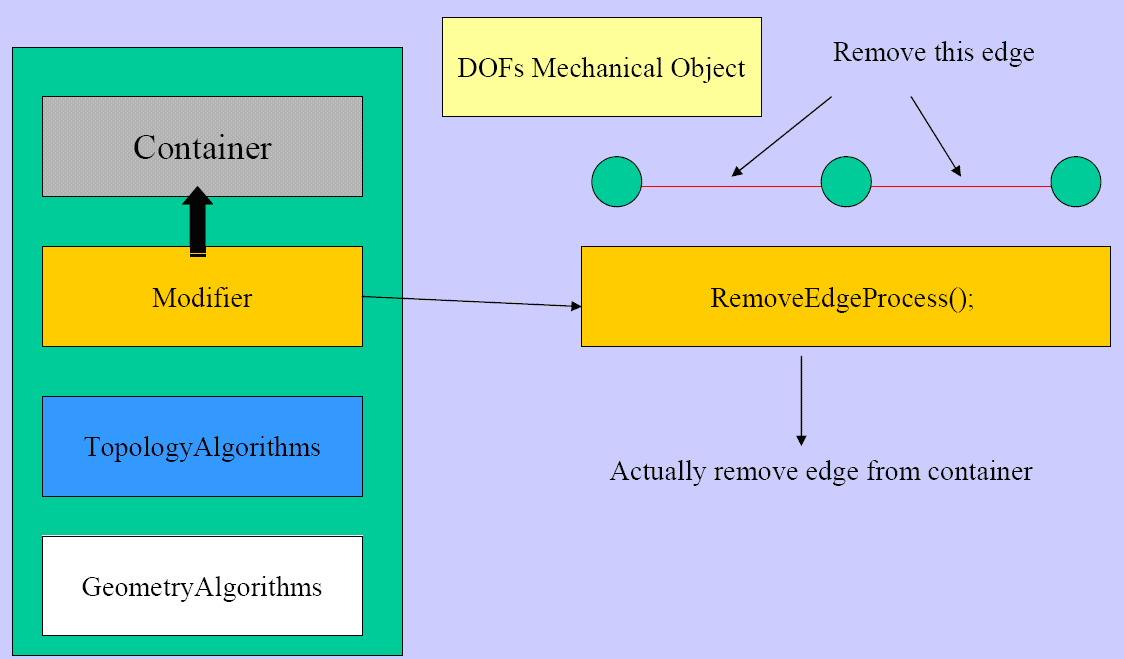
\includegraphics[width=0.95\linewidth]{Topology_Example_9}
  \caption{What happens when I split an Edge ? - Step 9.}
 \label{fig:Topology_Example_9}
\end{figure*}


\newpage
\section{Graphic User Interface}
\subsection{First steps}
\par
Once SOFA is compiled, in the directory bin will be placed an executable called runSofa (or runSofad if you are using the debug version).
The first time you will run SOFA, a GUI using Qt will appear. By default a simulation modeling a liver with some fixed points will be displayed. Simulations must be written in a xml format, generally, Sofa scenes have the extension ``.scn'', and Sofa objects directly the extension ``.xml''. You can load both of them using the file menu, or drag \& dropping them in the interface.\\
Basically the GUI is divided in two: 
\begin{itemize}
 \item a control panel subdivided in several tabulations, giving the user the possibility to display various information about the simulation, and even modifying it interactively
 \item a viewer: by default, you will be using our hand-made viewer, using OpenGL. Others are available, and below, we describe how to create your own viewer, if you desire to insert a more powerful rendering engine.
\end{itemize}

\begin{figure}[htpb]
	\centering
		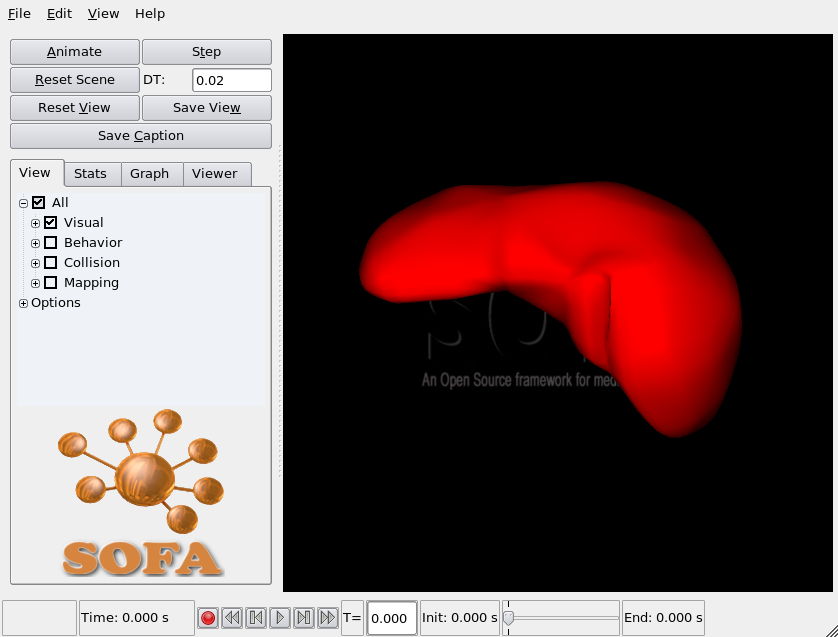
\includegraphics[width=1.0\textwidth]{GUI/GUI.png}
	\caption{SOFA first-time}
\end{figure}
At any time, you can hide the control panel by moving its right border to the left.
\newline

\par

\begin{figure}
	\centering
		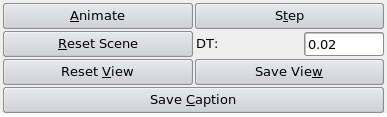
\includegraphics[width=0.45\textwidth]{GUI/GUI_basic.png}
	\caption{Basic Controls}
\end{figure}\begin{center}

\vspace{25mm}            \end{center}
The basics controls are :
\begin{itemize}
 \item {\bf Animate} : launch the simulation. The simulation won't stop until you press Animate.
 \item {\bf Step}: Process only one step of the simulation. 
 \item {\bf Reset Scene}: Reset all the components to their initial values.
 \item {\bf Reset View}: Reset the camera to its original place.
 \item {\bf Save View}: Save the position and orientation of the camera. Next time you will load your scene, these information will be used.
 \item {\bf Save Caption}: Take a screenshot of the current simulation.
\end{itemize}

DT corresponds to the time step used in the computation of the simulation. It can be changed interactively.










\subsection{View Tab}
The ``View Tab'' is the default tab, you can filter the information you want to be displayed by your viewer. It is quite useful to have a fast and global control. 

\begin{figure}[htpb]
	\centering
		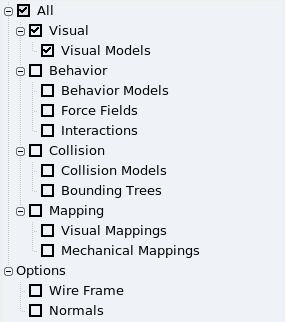
\includegraphics[width=0.3\textwidth]{GUI/GUI_visual.png}
	\caption{Basic Controls}
\end{figure}

The options are:
\begin{itemize}
 \item {\bf All}: Enable or disable the display of all the visual information available in SOFA
 \item {\bf Visual Models}: the graphic representation of the objects
\item {\bf Behavior Models}: the mechanical DOFs of the simulation
\item {\bf Collision Models}: the models used to perform the collision detection
\item {\bf Bounding Tree}: the hierarchical bounding boxes of the collision models
\item {\bf Mappings}: All the non-mechanical mappings (for instance the visual mappings that link a mechanical object to its visual representation)
\item {\bf Mechanical Mappings}: All the mechanical mapping that propagates the forces and position from a mechanical object to another
\item {\bf Interactions}: Interactions of all kind between objects. Some are created by the collision pipeline when a penalty response is used
\item {\bf Wire Frame}: Change the way 3D models(visual, and collision) are displayed
\item {\bf Normals}: Normals of the visual models
\end{itemize}








\subsection{Stats Tab}
The ``Stats Tab'' is a tab displaying an inventory of the collision models present in the scene( how many triangles, lines, points, spheres, are used to perform the collision detection). You can also output some information about the current simulation. 
\begin{itemize}
 \item Dump State: export in ``dumpState.data'' the state of the simulation
 \item Log Time: display in the console, the time spent in each step of the simulation. Useful to do some monitoring
 \item Gnuplot: export gnuplot files. It will export positions, velocities, energies. Files will have the same name as the Object associated in the simulation, following by:
\begin{itemize}
 \item {\bf ``\_x''} for the positions
 \item {\bf ``\_v''} for the velocities
 \item {\bf ``\_Energy''} for the Energies (contains kinetic, potential and mechanical)
\end{itemize}

You can specify the directory where you want the files to be saved in the menu Edit.
\end{itemize}











\subsection{Graph Tab}
The ``Graph tab'' is certainly the most important tab. It displays the scene graph of the simulation. You can quickly see all the components used in the current simulation. The ``Export Graph...'' button gives a graphic representation of the inter-dependencies of the objects.

\begin{figure}[htpb]
	\centering
		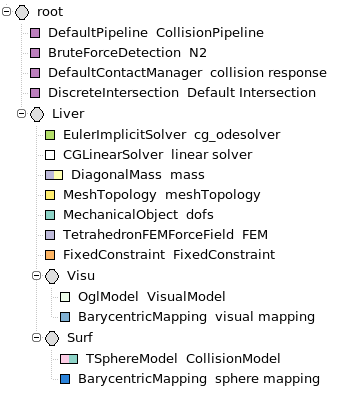
\includegraphics[width=0.5\textwidth]{GUI/GUI_graph.png}
	\caption{Scene Graph for the liver scene}
\end{figure}

This graph can dynamically change during the simulation: collisions can create new nodes, new components in case of contacts. But you can directly interact with it too. Double clicking on an item of the graph will make appear a small window displaying important data.

To know how to display the information of your brand new Sofa component, please refer to the section ``How to configure your Component''. Only objects of type ``sofa::core::objectmodel::Data'' or ``sofa::core::objectmodel::DataPtr'' can be displayed. It is important to understand that only these information will be kept if you decide to save the simulation. Loading a saved simulation, will just fill the components with this data.
This kind of dialog windows give the possibility to modify directly some characteristics of your component. Take care to click on the button ``Update'' once you have completed your modifications.

\begin{figure}[htpb]
	\centering
		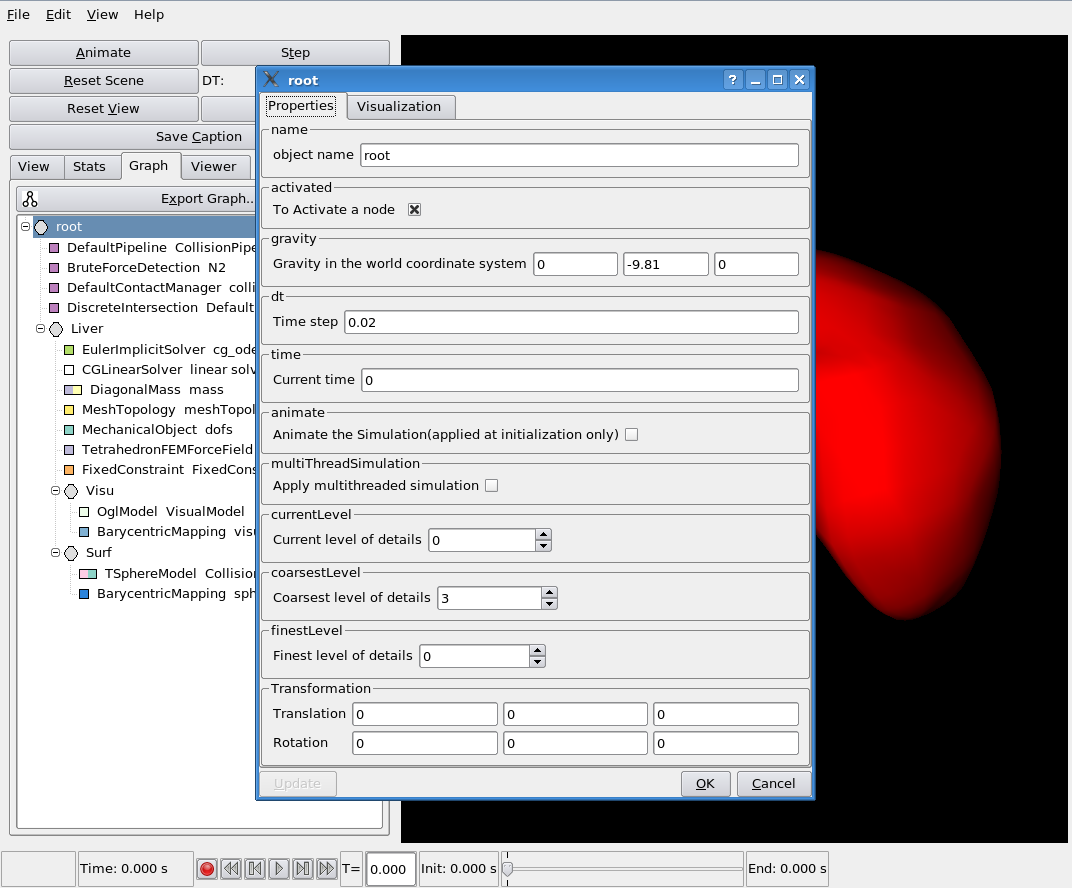
\includegraphics[width=0.8\textwidth]{GUI/GUI_modify.png}
	\caption{Double click on an item of the graph}
\end{figure}

\par
A Node gives access to much more interactions: right clicking on one of them makes appear a small context window.
\begin{itemize}
 \item {\bf Collapse}: Collapse the graph from the current node, close all the nodes below the clicked one
 \item {\bf Expand}: Expand the graph, and open all the nodes below the clicked one
 \item {\bf Desactivate}: Deactivate a part of the scene. Everything below this node won't be anymore taken into account. BUT it remains in the scene, and can be Activated again at any time
 \item {\bf Save Node}: Export in a XML files a part of the simulation
 \item {\bf Add Node}: Read a XML files describing an object or a whole scene, and put it right below the clicked node.
An interesting feature to note, is when you might be always using, and adding the same set of objects, you will find it convenient to add in the file scenes/object.txt the path to them. Like this, they will directly appear in the dialog window by default.
 \item {\bf Remove Node}: Remove from the simulation everything within the clicked node. You won't be able anymore to make it appear unless you proceed to a restart or reload of the scene.
 \item {\bf Modify}: Open the same dialog window as might do a double click: this action is common to all the items of the graph
\end{itemize}

\begin{figure}[htpb]
	\centering
		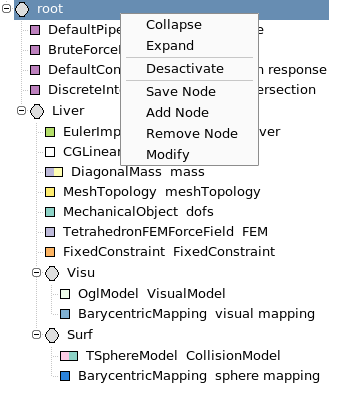
\includegraphics[width=0.4\textwidth]{GUI/GUI_interaction.png}
	\caption{Right click on a node of the graph}
\end{figure}








\subsection{Viewer Tab}
The ``Viewer tab'' describes all the keyboard shortcuts available for the current viewer.

The last useful option of this tab is the possibility to re-size your viewer, which can be very helpful to record a video at a given resolution.









\subsection{Interactions}
You can interact with the simulation using the mouse with SHIFT + Right Click. A ray will be cast, and if it intersects one collision model of the scene, a spring will be created, allowing you to pull on some elements of the scene.



\newpage
\subsection{Architecture}
Fig.~\ref{fig:GUI_UML} gives an overview of the modular architecture of the GUI for SOFA. 
\begin{figure}[htpb]
	\centering
		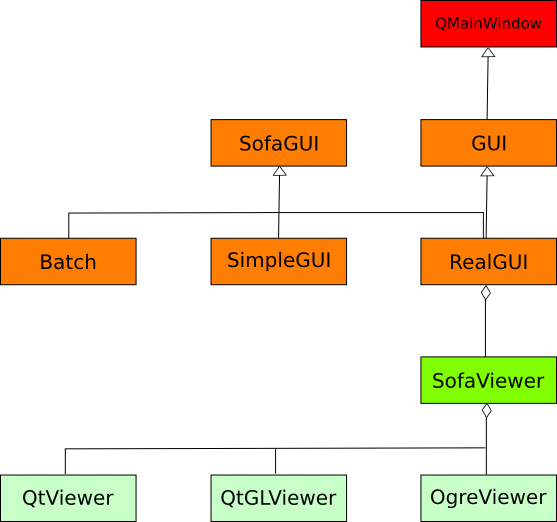
\includegraphics[width=0.9\textwidth]{GUI/GUI_UML.png}
	\caption{A modular Architecture of the GUI}
 	\label{fig:GUI_UML}
\end{figure}








\subsection{Change the viewer}
By default, SOFA provides three viewers, that can be integrated easily to the Qt interface. 

\begin{itemize}
 \item {\bf QtViewer}: a hand made viewer using OpenGL functionality
 \item {\bf QtGLViewer}: a viewer using the library QGLViewer created by Gilles Debunne. It is distributed directly with SOFA, but you can also download it at:\\ {\bf http://artis.imag.fr/Members/Gilles.Debunne/QGLViewer/}
 \item {\bf OgreViewer}: this viewer remains experimental, but shows how it is possible to integrate a powerful rendering engine such as OGRE3D. You need to install Ogre. You can download it at {\bf http://www.ogre3d.org}.
\end{itemize}

To use them, you have to edit the file sofa-default.cfg located in your SOFA directory, and uncomment the lines corresponding to the viewer you want. If you have several viewers activated, you can launch SOFA with a specific one by using the option:
\begin{itemize}
 \item ``runSofa -g qt'' : for QtViewer
 \item ``runSofa -g qglviewer'' : for QtGLViewer
 \item ``runSofa -g ogre'' : for OgreViewer
\end{itemize}

You can also dynamically change the viewer when SOFA is running. The menu View of the main window displays all the viewer available and let you switch at any time.
\par
If you desire to create a new viewer, the first step is to make it derive from SofaViewer. 








\subsection{Choose the GUI}
By default, Sofa provides three GUIs.
\begin{itemize}
 \item {\bf Batch}: no gui, proceeds to 1000 iterations and then stops
 \item {\bf GLUT}: GLUT window, implementing only the basic functions. To start the animation, you have to pass the option ``-s'' to your runSofa
 \item {\bf Qt}: the default GUI, already described above
\end{itemize}

The Batch GUI is always available. To use GLUT or Qt interface, you have to uncomment in sofa-default.cfg the corresponding lines. To use them
\begin{itemize}
 \item ``runSofa -g batch'' : for no GUI
 \item ``runSofa -g glut'' : for GLUT window 
 \item for Qt GUI, please refer to the section above. By default, Sofa is using Qt interface with QtViewer.
\end{itemize}
If you desire to create a new GUI, the first step is to make it derive from SofaGUI. 






\subsection{Player/Recorder}

\begin{figure}[htpb]
	\centering
		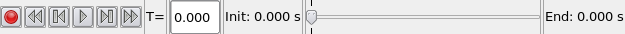
\includegraphics[width=0.7\textwidth]{GUI/GUI_recorder.png}
	\caption{Player/Recorder in Sofa} 	
\end{figure}
Sofa provides with the Qt Graphic interface, a compact Player/Recorder of simulation. When you want to record a simulation, press the red button (record). Automatically, some components will be added to your graph, and will create files to save the position, and velocities of all your mechanical elements. To stop recording, press again on the record button. A file with the same name as your simulation will be created, but with the extension ``.simu''. Sofa is able to read these files, and will initialize correctly the Player. 
\par
To readback a recorded simulation, you can process to a step by step(forward, and backward), or a continuous play. You can jump to a specific moment of your recording. You can even change the Dt of the recording, if you want to accelerate, or reduce the velocity of the playing. At any time, you can animate the scene (by pressing the Animate button), to compute the simulation. 
\par
The files will be stored by default in the directory scenes/simulation of your SOFA. Nevertheless, you can change this directory by clicking on the menu Edit of the main window.







\section{Modeler}
A modeler for Sofa has been recently created. The purpose of this tool is both to help the new-comers in Sofa to get an overview of the whole framework, and accelerate the process of creation and configuration of a complex simulation for expert users.
\begin{figure}[htpb]
	\centering
		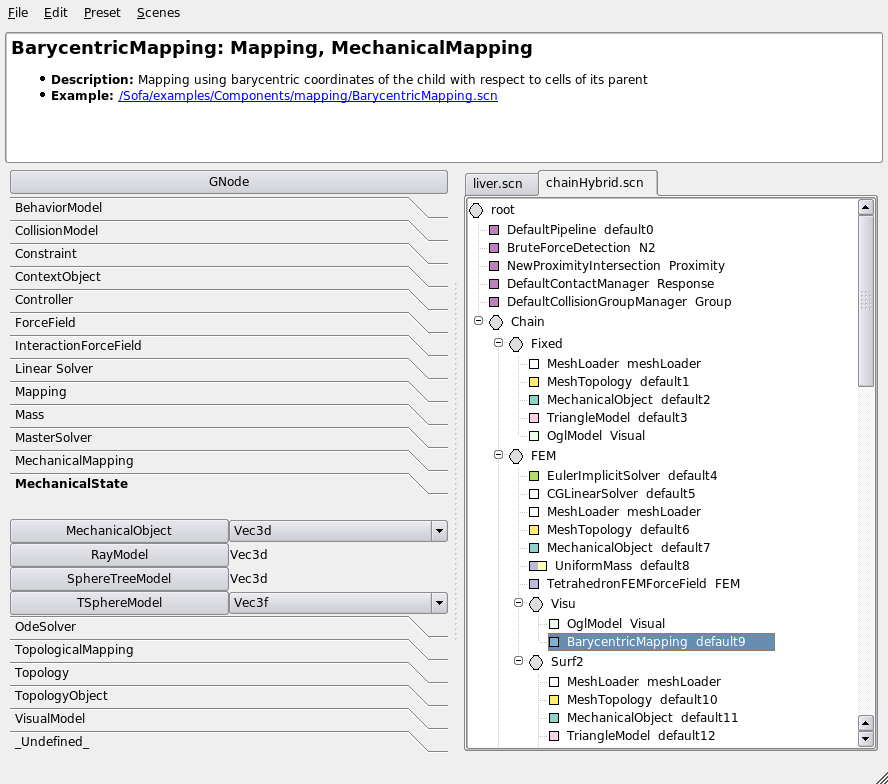
\includegraphics[width=0.75\textwidth]{GUI/Modeler.png}
	\caption{Main Window of the Modeler} 	
\end{figure}

\subsection{Library}
The left part of the application displays a library of all the different components available in Sofa, sorted by the name of the Base Class. Clicking on any of them will display information about the usage, authors, licence if any, and sometimes a link to an example. This link will open a new tab in the modeler displaying a simulation. 
At any time, you can launch Sofa from the Modeler, hitting CTRL+R, or going to File ... Run In Sofa.
\subsection{Graph Editor}
The right part seems very similar to the scene graph displayed in Sofa. The behavior is the same. Double clicking on a component will open a dialog, in which you can define all the parameters of the object. But, as you are in an editor, you can easily remove everything you have added. This editor is very convenient to test things. Try to create your object, launch into sofa, modify some components, or parameters, using the documentation displayed each time you select one item. 
\subsection{Modeling}
To model a new scene, just make a series of drag and drop of the components you desire from the Library to the Graph Editor. By default, when opening a new tab, all the default components to perform the collision detection are added. If you don't want them, just clear the tab (CTRL+N).\\
To accelerate the process of creation, preset objects are available. You can build automatically :
\begin{itemize}
  \item deformable objects
  \begin{itemize}
    \item in a grid
    \item using a tetrahedral mesh
  \end{itemize}
  \item rigid objects  
  \begin{itemize}
    \item simulated
    \item not simulated: they will perform as obstacle like floors, or walls
  \end{itemize}
\end{itemize}



\newpage

\section{Light management}

One white global light illuminates the scene by default. This can be changed
through a light manager object and a certain number of lights (limited by
OpenGL).

The first step is to add the object called ``LightManager'', preferably at the
top of the scene file.
\begin{code_xml}
	<Object type=``LightManager'' />
\end{code_xml}

After that, we can add 3 different kinds of lights :
\begin{itemize}
  \item a positional light (parameters : color, position) ;
	\begin{figure}[!h]
	\centering
	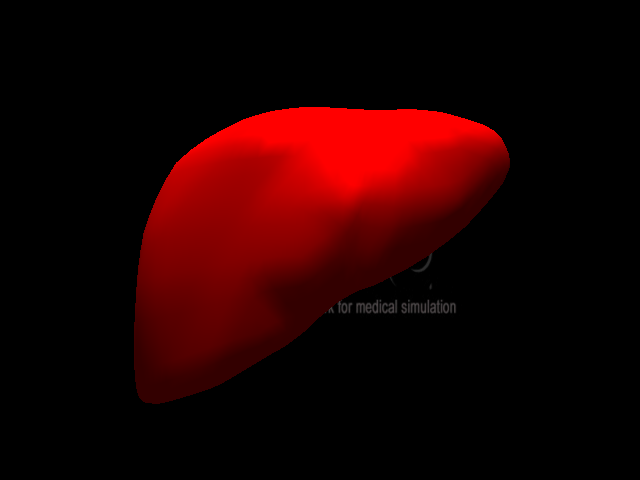
\includegraphics[width=0.33\linewidth]{rendering/images/light_pos.png}
	\caption{Positional Light}
	\end{figure}

	\begin{code_xml}
		<Object type="PositionalLight" position="0 -5 10" />
	\end{code_xml}
%\newpage
  \item a directional light (parameters : color, direction) ; 
	\begin{figure}[!h]
	\centering
	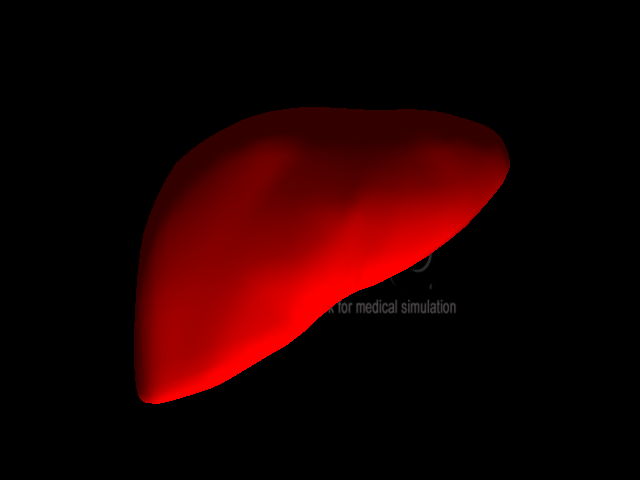
\includegraphics[width=0.33\linewidth]{rendering/images/light_dir.png}
	\caption{Directional Light}
	\end{figure}

	\begin{code_xml}
		<Object type="DirectionalLight" direction="0 5 0" />
	\end{code_xml}
\newpage

  \item and a spotlight (parameters : color, position, direction, cut off,
  exponent, attenuation)

	\begin{figure}[!h]
	\centering
	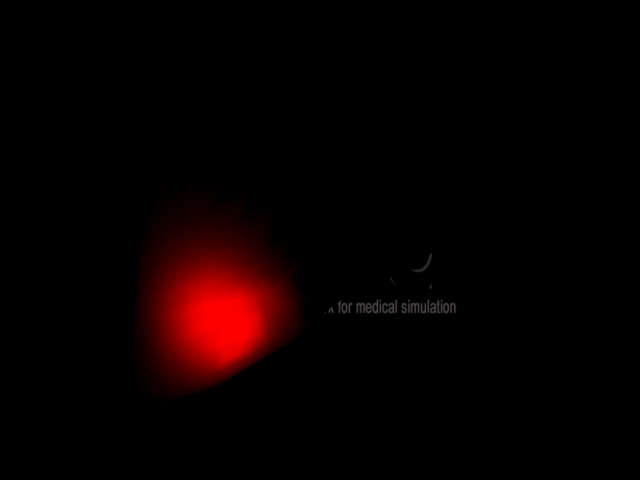
\includegraphics[width=0.33\linewidth]{rendering/images/light_spot.png}
	\caption{Spot Light}
	\end{figure}

	\begin{code_xml}
		<Object type="SpotLight" position="-3 2 5" direction="0 0 -1" />
	\end{code_xml}
\end{itemize}

\section{Shader management}
A complete set of tools about using shaders is implemented into SOFA. The three kinds of shaders (vertex and fragments (mandatory), geometry (optionally)) are available.
Shader is used only for Visual Model as OglModel.
\newline
The effects of the shader is spread to the associated subtree.
Finally, there is only one shader activated for each visual model : if two shaders are present in the same node, only the second will be effective.

	\begin{figure}[!h]
	\centering
	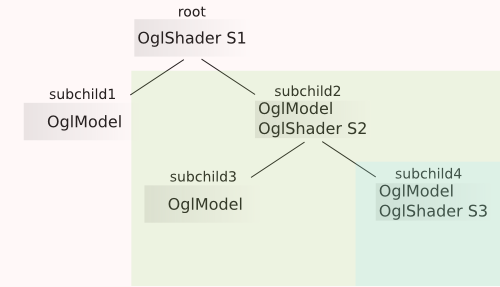
\includegraphics[width=0.8\linewidth]{rendering/images/shader_tree.png}
	\caption{Example of shaders' area of effect}
	\end{figure}

To simply include a shader, add this into your node :
	\begin{code_xml}
		<Object type="OglShader" vertFilename=``test.vert'' fragFilename=``test.frag'' />
	\end{code_xml}

\textit{vertFilename} and \textit{fragFilename} are the only mandatory parameters. Other optional parameters are about geometry shader : \textit{geoFilename}, \textit{geometryInputType}, \textit{geometryOutputType} and \textit{geometryVerticesOut}. A last parameter, \textit{turnOn}, is for debugging purpose, when you want to disable shader without restarting the scene.

If you want to send values to uniform varaibles defined into the shader, a certain number of objects is available : 
\begin{itemize}
 \item OglIntVariable,OglInt{2,3,4}Variable : for int and ivec{2,3,4}
 \item OglFloatVariable,OglFloat{2,3,4}Variable : for float and vec{2,3,4}
 \item OglIntVectorVariable, OglIntVector{2,3,4}Variable : for arrays of int and ivec{2,3,4}
 \item OglFloatVectorVariable, OglFloatVector{2,3,4}Variable : for arrays of float and vec{2,3,4}
\end{itemize}

Their parameters are \textit{id} for their name into the shader and \textit{value} (single type) or \textit{values} (array type).
Example : 
	\begin{code_xml}
		<Object type="OglFloat3Variable" id="fragmentColor" value="1.0 0.0 0.0" />
		<Object type="OglFloatVariable" id="fragmentOpacity" value="2.0"/>
		<Object type="OglFloatVector4Variable" id="MappingTable" values="1.0 0.0 0.0 0.0 0.0 0.0 0.0 1.0" />
	\end{code_xml}

2D texture can be added with OglTexture2D object.Its parameters are \textit{id}, \textit{texture2DFilename} and \textit {textureUnit}.

	\begin{code_xml} 
		<Object type="OglTexture2D" texture2DFilename="textures/lights4-small-noise.bmp" textureUnit="1" id="planeTexture" />
	\end{code_xml}

The last object about shaders is a partial support of macro processing in GLSL. It's possible to define macro variable if a part of code is enabled or not. For example, this can be very useful if there is a common code for two 3D objects, one with a texture, and the other with simple colors. You define the macro :

	\begin{code_cpp} 
		#define HAS_TEXTURE
			...;
			//code about textured 3D object
		#else
			...;
			//code about colored 3D object
		#endif
	\end{code_cpp}

and put the following object into the scene file, at the same node as the OglShader used by the textured 3D object:

	\begin{code_xml} 
		<Object type="OglShaderDefineMacro" id="HAS_TEXTURE" />
	\end{code_xml}




% This chapter is defined here
\chapter{How to contribute to this documentation}
\section{Document structure}
This document gathers the content of other documents located in different subdirectories. These documents can also be compiled as stand-alone documents.
The structure can be illustrated as follows:
\begin{itemize}
 \item \texttt{sofadocumentation.tex} : the root document.
 \item \texttt{macros\_docu.tex} : custom commands and macros. This file is included by the root document.
 \item \texttt{introduction} : a subdirectory containing a chapter of this document.
\begin{itemize}
 \item \texttt{introduction.tex} : a stand-alone article containing the same. This file may include \texttt{../macros\_docu.tex} to use the common custom commands.
 \item \texttt{introduction\_body.tex} : the text of the chapter/article. This file is included as a chapter by \texttt{sofadocumentation.tex}, and included as full article text by \texttt{introduction.tex}.
\end{itemize}
 \item there could (and hopefully will !) be other subdirectories with a similar structure.
\end{itemize}

\section{Compiling the document}
\subsection{File formats}
The graphics are handled by: \texttt{\textbackslash usepackage[pdftex]\{graphicx\}}. This allows the inclusion of \texttt{.png} images rather than \texttt{.eps}, which makes the image files much smaller, and compilation of \texttt{html} faster. The result of the compilation is a \texttt{.pdf} rather than a \texttt{.dvi} file.

\subsection{Include paths}
The root document includes files in the subdirectories, which in turn include files too. The problem is that the path from the subdirectory (used when compiling a stand-alone article) is not the same as from the parent directory (used when compiling the whole report).
It seems that \LaTeX has no include path command to circumvent this problem.

Fortunately, \LaTeX uses an environment variable named TEXINPUTS which represents a list of directories to search. We use this variable to allow file inclusion, by adding the parent directories to the list. The command lines depend on the shell, e.g.:
\begin{itemize}
 \item using bash: \texttt{export TEXINPUTS=\$\{TEXINPUTS\}:..:../.. ; latex sofadocumentation.tex}
 \item using tcsh: \texttt{setenv TEXINPUTS \$\{TEXINPUTS\}:..:../.. ; latex sofadocumentation.tex}
\end{itemize}

Using the \texttt{Kile} graphical front-end, you can customize the command line in menu \texttt{Settings/Kile/Tools/Build}, select tool \texttt{LATEX} and write the appropriate command line in the \texttt{Command} field.

\subsection{HTML}
HTML can be generated using the following command:\\
\texttt{latex2html sofadocumentation.tex -mkdir -dir ./html -show\_section\_numbers -split 1}
\\
Currently, the listings do not appear in html.

\end{document}          
